\documentclass[]{article}
\usepackage{lmodern}
\usepackage{amssymb,amsmath}
\usepackage{bm}
\usepackage{soul}
\usepackage[color=yellow]{todonotes}
\usepackage{ifxetex,ifluatex}
\usepackage{fixltx2e} % provides \textsubscript
\ifnum 0\ifxetex 1\fi\ifluatex 1\fi=0 % if pdftex
  \usepackage[T1]{fontenc}
  \usepackage[utf8]{inputenc}
\else % if luatex or xelatex
  \ifxetex
    \usepackage{mathspec}
  \else
    \usepackage{fontspec}
  \fi
  \defaultfontfeatures{Ligatures=TeX,Scale=MatchLowercase}
\fi
% use upquote if available, for straight quotes in verbatim environments
\IfFileExists{upquote.sty}{\usepackage{upquote}}{}
% use microtype if available
\IfFileExists{microtype.sty}{%
\usepackage{microtype}
\UseMicrotypeSet[protrusion]{basicmath} % disable protrusion for tt fonts
}{}
\usepackage[margin=1in]{geometry}
\usepackage{hyperref}
\hypersetup{unicode=true,
            pdftitle={13 Time series models with covariates, and a case study of polio},
            pdfauthor={Edward Ionides},
            pdfborder={0 0 0},
            breaklinks=true}
\urlstyle{same}  % don't use monospace font for urls
\usepackage{color}
\usepackage{fancyvrb}
\newcommand{\VerbBar}{|}
\newcommand{\VERB}{\Verb[commandchars=\\\{\}]}
\DefineVerbatimEnvironment{Highlighting}{Verbatim}{commandchars=\\\{\}}
% Add ',fontsize=\small' for more characters per line
\usepackage{framed}
\definecolor{shadecolor}{RGB}{248,248,248}
\newenvironment{Shaded}{\begin{snugshade}}{\end{snugshade}}
\newcommand{\KeywordTok}[1]{\textcolor[rgb]{0.13,0.29,0.53}{\textbf{#1}}}
\newcommand{\DataTypeTok}[1]{\textcolor[rgb]{0.13,0.29,0.53}{#1}}
\newcommand{\DecValTok}[1]{\textcolor[rgb]{0.00,0.00,0.81}{#1}}
\newcommand{\BaseNTok}[1]{\textcolor[rgb]{0.00,0.00,0.81}{#1}}
\newcommand{\FloatTok}[1]{\textcolor[rgb]{0.00,0.00,0.81}{#1}}
\newcommand{\ConstantTok}[1]{\textcolor[rgb]{0.00,0.00,0.00}{#1}}
\newcommand{\CharTok}[1]{\textcolor[rgb]{0.31,0.60,0.02}{#1}}
\newcommand{\SpecialCharTok}[1]{\textcolor[rgb]{0.00,0.00,0.00}{#1}}
\newcommand{\StringTok}[1]{\textcolor[rgb]{0.31,0.60,0.02}{#1}}
\newcommand{\VerbatimStringTok}[1]{\textcolor[rgb]{0.31,0.60,0.02}{#1}}
\newcommand{\SpecialStringTok}[1]{\textcolor[rgb]{0.31,0.60,0.02}{#1}}
\newcommand{\ImportTok}[1]{#1}
\newcommand{\CommentTok}[1]{\textcolor[rgb]{0.56,0.35,0.01}{\textit{#1}}}
\newcommand{\DocumentationTok}[1]{\textcolor[rgb]{0.56,0.35,0.01}{\textbf{\textit{#1}}}}
\newcommand{\AnnotationTok}[1]{\textcolor[rgb]{0.56,0.35,0.01}{\textbf{\textit{#1}}}}
\newcommand{\CommentVarTok}[1]{\textcolor[rgb]{0.56,0.35,0.01}{\textbf{\textit{#1}}}}
\newcommand{\OtherTok}[1]{\textcolor[rgb]{0.56,0.35,0.01}{#1}}
\newcommand{\FunctionTok}[1]{\textcolor[rgb]{0.00,0.00,0.00}{#1}}
\newcommand{\VariableTok}[1]{\textcolor[rgb]{0.00,0.00,0.00}{#1}}
\newcommand{\ControlFlowTok}[1]{\textcolor[rgb]{0.13,0.29,0.53}{\textbf{#1}}}
\newcommand{\OperatorTok}[1]{\textcolor[rgb]{0.81,0.36,0.00}{\textbf{#1}}}
\newcommand{\BuiltInTok}[1]{#1}
\newcommand{\ExtensionTok}[1]{#1}
\newcommand{\PreprocessorTok}[1]{\textcolor[rgb]{0.56,0.35,0.01}{\textit{#1}}}
\newcommand{\AttributeTok}[1]{\textcolor[rgb]{0.77,0.63,0.00}{#1}}
\newcommand{\RegionMarkerTok}[1]{#1}
\newcommand{\InformationTok}[1]{\textcolor[rgb]{0.56,0.35,0.01}{\textbf{\textit{#1}}}}
\newcommand{\WarningTok}[1]{\textcolor[rgb]{0.56,0.35,0.01}{\textbf{\textit{#1}}}}
\newcommand{\AlertTok}[1]{\textcolor[rgb]{0.94,0.16,0.16}{#1}}
\newcommand{\ErrorTok}[1]{\textcolor[rgb]{0.64,0.00,0.00}{\textbf{#1}}}
\newcommand{\NormalTok}[1]{#1}
\usepackage{graphicx,grffile}
\makeatletter
\def\maxwidth{\ifdim\Gin@nat@width>\linewidth\linewidth\else\Gin@nat@width\fi}
\def\maxheight{\ifdim\Gin@nat@height>\textheight\textheight\else\Gin@nat@height\fi}
\makeatother
% Scale images if necessary, so that they will not overflow the page
% margins by default, and it is still possible to overwrite the defaults
% using explicit options in \includegraphics[width, height, ...]{}
\setkeys{Gin}{width=\maxwidth,height=\maxheight,keepaspectratio}
\IfFileExists{parskip.sty}{%
\usepackage{parskip}
}{% else
\setlength{\parindent}{0pt}
\setlength{\parskip}{6pt plus 2pt minus 1pt}
}
\setlength{\emergencystretch}{3em}  % prevent overfull lines
\providecommand{\tightlist}{%
  \setlength{\itemsep}{0pt}\setlength{\parskip}{0pt}}
%\setcounter{secnumdepth}{0}
\setcounter{section}{13}
% Redefines (sub)paragraphs to behave more like sections
\ifx\paragraph\undefined\else
\let\oldparagraph\paragraph
\renewcommand{\paragraph}[1]{\oldparagraph{#1}\mbox{}}
\fi
\ifx\subparagraph\undefined\else
\let\oldsubparagraph\subparagraph
\renewcommand{\subparagraph}[1]{\oldsubparagraph{#1}\mbox{}}
\fi

%%% Use protect on footnotes to avoid problems with footnotes in titles
\let\rmarkdownfootnote\footnote%
\def\footnote{\protect\rmarkdownfootnote}

%%% Change title format to be more compact
\usepackage{titling}

% Create subtitle command for use in maketitle
\newcommand{\subtitle}[1]{
  \posttitle{
    \begin{center}\large#1\end{center}
    }
}

\setlength{\droptitle}{-2em}
  \title{13. Time series models with covariates, and a case study of polio}
  \pretitle{\vspace{\droptitle}\centering\huge}
  \posttitle{\par}
  \author{Edward Ionides}
  \preauthor{\centering\large\emph}
  \postauthor{\par}
  \predate{\centering\large\emph}
  \postdate{\par}
  \date{04/08/2018}


\begin{document}
\maketitle

{
\setcounter{tocdepth}{2}
\tableofcontents
}
\newcommand\prob{\mathbb{P}}
\newcommand\E{\mathbb{E}}
\newcommand\var{\mathrm{Var}}
\newcommand\cov{\mathrm{Cov}}
\newcommand\loglik{\ell}
\newcommand\R{\mathbb{R}}
\newcommand\data[1]{#1^*}
\newcommand\params{\, ; \,}
\newcommand\transpose{\scriptsize{T}}
\newcommand\eqspace{\quad\quad}
\newcommand\myeq[1]{\eqspace \displaystyle #1}
\newcommand\lik{\mathcal{L}}
\newcommand\profileloglik[1]{\ell^\mathrm{profile}_#1}
\newcommand\ar{\phi}
\newcommand\ma{\psi}
\newcommand\AR{\Phi}
\newcommand\MA{\Psi}
\newcommand\ev{u}
\newcommand\given{{\, | \,}}
\newcommand\equals{{=\,}}
\newcommand\matA{\mathbb{A}}
\newcommand\matB{\mathbb{B}}
\newcommand\matH{\mathbb{H}}
\newcommand\covmatX{\mathbb{U}}
\newcommand\covmatY{\mathbb{V}}




\begin{center}\rule{0.5\linewidth}{\linethickness}\end{center}

Produced with R version 3.4.3 and \textbf{pomp} version 1.16.

\begin{center}\rule{0.5\linewidth}{\linethickness}\end{center}

Objectives

\begin{enumerate}
\def\labelenumi{\arabic{enumi}.}
\item
  Discuss covariates in POMP models as a generalization of regression
  with ARMA errors.
\item
  Demonstrate the use of covariates in \textbf{pomp} to add demographic
  data (birth rates and total population) and seasonality to an
  epidemiological model.
\item
  Present a case study, developing and fitting a POMP model with
  covariates.
\end{enumerate}

\begin{center}\rule{0.5\linewidth}{\linethickness}\end{center}

\begin{center}\rule{0.5\linewidth}{\linethickness}\end{center}

\subsection{Covariates in time series
analysis}\label{covariates-in-time-series-analysis}

\begin{itemize}
\item
  Suppose our time series of primary interest is \(\data{y_{1:N}}\).
\item
  A \textbf{covariate} time series is an additional time series
  \({z_{1:N}}\) which is used to help explain \(\data{y_{1:N}}\).
\item
  When we talk about covariates, it is often implicit that we think of
  \({z_{1:N}}\) as a measure of an \textbf{external forcing} to the
  system producing \(\data{y_{1:N}}\). This means that the process
  generating the data \({z_{1:N}}\) affects the process generating
  \(\data{y_{1:N}}\), but not vice versa.

  \begin{itemize}
  \tightlist
  \item
    For example, the weather might affect human health, but human health
    has negligible effect on weather: weather is an external forcing to
    human health processes.
  \end{itemize}
\item
  When we make an assumption of external forcing, we should try to make
  it explicit.
\item
  In regression analysis, we usually \textbf{condition} on covariates.
  Equivalently, we model them as fixed numbers, rather than modeling
  them as the outcome of random variables.
\item
  When the process leading to \({z_{1:N}}\) is not external to the
  system generating it, we must be alert to the possibility of
  \textbf{reverse causation} and \textbf{confounding variables}. Further
  discussion of this issue, in the context of a time series analysis, is
  given in the case study on
  \href{http://ionides.github.io/531w16/notes10/notes10.html\#conclusions}{An
  association between unemployment and mortality?}.
\item
  Isses involved in inferring causation from fitting statistical models
  are essentially the same whether the model is linear and Gaussian or
  not.
\end{itemize}

\begin{center}\rule{0.5\linewidth}{\linethickness}\end{center}

\begin{center}\rule{0.5\linewidth}{\linethickness}\end{center}

\subsubsection{Covariates in linear time series
analysis}\label{covariates-in-linear-time-series-analysis}

\begin{itemize}
\item
  The main tool we have seen previously for investigating dependence on
  covariates is regression with ARMA errors.
\item
  This tool can also be used to identify lag relationships, where
  \(\data{y_{n}}\) depends on \(z_{n-L}\).

  \begin{itemize}
  \tightlist
  \item
    An example of identifying lag in the midterm project:
    \href{https://ionides.github.io/531w16/midterm_project/project20/midterm.html\#try-other-lags}{The
    relationship between S\&P500 and CPI}.
  \end{itemize}
\item
  Another way to investigate associations at different lags is by
  computing the sample correlation between \(\data{y_n}\) and
  \(z_{n-L}\), for \(n\in L+1:N\), and plotting this against \(L\).
\item
  This is called the \textbf{cross-correlation function} and can be
  computed with the R function \texttt{ccf}.

  \begin{itemize}
  \tightlist
  \item
    An example of the use of the cross-correlation function in a midterm
    project:
    \href{https://ionides.github.io/531w16/midterm_project/project3/midterm_project.html}{The
    Association between Recent Cholera Epidemics and Rainfall in Haiti}.
  \end{itemize}
\end{itemize}

\begin{center}\rule{0.5\linewidth}{\linethickness}\end{center}

\begin{center}\rule{0.5\linewidth}{\linethickness}\end{center}

\subsubsection{Covariates in nonlinear POMP
models}\label{covariates-in-nonlinear-pomp-models}

\begin{itemize}
\item
  Time series modeling of regression errors is only one of many ways in
  which covariates could be used to explain a dynamic system.
\item
  In general, it is nice if scientific considerations allow you to
  propose sensible ways to model the relationship.

  \begin{itemize}
  \item
    In an epidemiological model for malaria, rainfall might affect the
    number of mosquitoes (and hence the disease transmission rate) but
    not the duration of infection.
  \item
    In an economic model, geopolitical shocks to the oil supply might
    have direct influence on energy prices, secondary direct effects on
    inflation and investment, and indirect consequences for
    unemployment.
  \item
    In a hydrology model, precipitation is a covariate explaining river
    flow, but the exact nature of the relationship is a question of
    interest.
  \end{itemize}
\item
  The general POMP modeling framework allows essentially arbitrary
  modeling of covariates.
\item
  Recall that a POMP model is specified by defining the following:
  \[\begin{array}{l}
  f_{X_{0}}(x_0\params\theta),
  \\
  f_{X_{n}|X_{n-1}}(x_{n}\given x_{n-1}\params\theta),
  \\
  f_{Y_{n}|X_n}(y_{n}\given x_n\params\theta),
  \end{array}\] for \(n=1:N\)
\item
  The possibility of a general dependence on \(n\) includes the
  possibility that there is some covariate time series \(z_{0:N}\) such
  that \[\begin{array}{lcl}
  f_{X_{0}}(x_0\params\theta)&=& f_{X_{0}}(x_0\params\theta,z_0)
  \\
  f_{X_{n}|X_{n-1}}(x_{n}\given x_{n-1}\params\theta) &=& f_{X_{n}|X_{n-1}}(x_{n}\given x_{n-1}\params\theta,z_n),
  \\
  f_{Y_{n}|X_n}(y_{n}\given x_n\params\theta) &=& f_{Y_{n}|X_n}(y_{n}\given x_n\params\theta,z_n),
  \end{array}\] for \(n=1:N\)
\item
  One specific choice of covariates is to construct \(z_{0:N}\) so that
  it fluctuates periodically, once per year. This allows
  \textbf{seasonality} enter the POMP model in whatever way is
  appropriate for the system under investigation.
\item
  All that remains is to hypothesize what is a reasonable way to include
  covariates for your system, and to implement the resulting data
  analysis.
\item
  The \textbf{pomp} package provides facilities for including covariates
  in a pomp object, and making sure that the covariates are accessible
  to \texttt{rprocess}, \texttt{dprocess}, \texttt{rmeasure},
  \texttt{dmeasure}, and the state initialization at time \(t_0\).
\item
  Named covariate time series entered via the \texttt{covar} argument to
  \texttt{pomp} are automatically defined within Csnippets used for the
  \texttt{rprocess}, \texttt{dprocess}, \texttt{rmeasure},
  \texttt{dmeasure} and \texttt{initializer} arguments.
\item
  Let's see this in practice, using population census, birth data and
  seasonality as covariates in an epidemiological model.
\end{itemize}

\begin{center}\rule{0.5\linewidth}{\linethickness}\end{center}

\begin{center}\rule{0.5\linewidth}{\linethickness}\end{center}

\subsection{Case study: polio in
Wisconsin}\label{case-study-polio-in-wisconsin}

\begin{itemize}
\item
  The massive global polio eradication initiative (GPEI) has brought
  polio from a major global disease to the brink of extinction.
\item
  Finishing this task is proving hard, and improved understanding polio
  ecology might assist.
\item
  Martinez-Bakker et al. (2015) investigated this using extensive state
  level pre-vaccination era data in USA.
\item
  We will follow the approach of Martinez-Bakker et al. (2015) for one
  state (Wisconsin). In the context of their model, we can quantify
  seasonality of transmission, the role of the birth rate in explaining
  the transmission dynamics, and the persistence mechanism of polio.
\item
  Martinez-Bakker et al. (2015) carrried out this analysis for all 48
  contigous states and District of Columbia, and their data and code are
  publicly available. The data we study, in \url{polio_wisconsin.csv},
  consist of \texttt{cases}, the monthly reported polio cases;
  \texttt{births}, the monthly recorded births; \texttt{pop}, the annual
  census; \texttt{time}, date in years.
\end{itemize}

\begin{Shaded}
\begin{Highlighting}[]
\NormalTok{polio_data <-}\StringTok{ }\KeywordTok{read.table}\NormalTok{(}\StringTok{"polio_wisconsin.csv"}\NormalTok{)}
\KeywordTok{colnames}\NormalTok{(polio_data)}
\end{Highlighting}
\end{Shaded}

\begin{verbatim}
## [1] "time"   "cases"  "births" "pop"
\end{verbatim}

\begin{itemize}
\item
  We implement the compartment model of Martinez-Bakker et al. (2015),
  having compartments representing susceptible babies in each of six
  one-month birth cohorts (\(S^B_1\),\ldots{},\(S^B_6\)), susceptible
  older individuals (\(S^O\)), infected babies (\(I^B\)), infected older
  individuals (\(I^O\)), and recovered with lifelong immunity (\(R\)).
\item
  The state vector of the disease transmission model consists of numbers
  of individuals in each compartment at each time,
  \[X(t)=\big(S^B_1(t),...,S^B_6(t), I^B(t),I^O(t),R(t) \big).\]
\item
  Babies under six months are modeled as fully protected from
  symptomatic poliomyelitis; older infections lead to reported cases
  (usually paralysis) at a rate \(\rho\).
\item
  The flows through the compartments are graphically represented as
  follows (Figure 1A of Martinez-Bakker et al. (2015)):
\end{itemize}

\begin{figure}
\centering
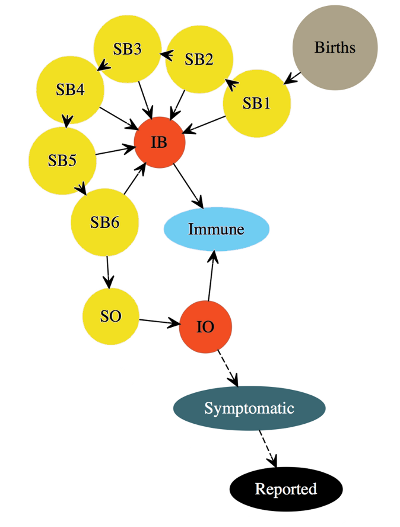
\includegraphics{./polio_fig1A.png}
\caption{Polio model diagram}
\end{figure}

\begin{itemize}
\item
  Since duration of infection is comparable to the one-month reporting
  aggregation, a discrete time model may be appropriate. Martinez-Bakker
  et al. (2015) fitted monthly observations from May 1932 through
  January 1953, so we define \(t_n=1932+ (4+n)/12\) for \(n=0,\dots,N\),
  and we write
  \[X_n=X(t_n)=\big(S^B_{1,n},...,S^B_{6,n}, I^B_n,I^O_n,R_n \big).\]
\item
  The mean force of infection, in units of \(\mathrm{yr}^{-1}\), is
  modeled as
  \[\bar\lambda_n=\left( \beta_n \frac{I^O_n+I^B_n}{P_n} + \psi \right)\]
  where \(P_n\) is census population interpolated to time \(t_n\) and
  seasonality of transmission is modeled as
  \[\beta_n=\exp\left\{ \sum_{k=1}^K b_k\xi_k(t_n) \right\},\] with
  \(\{\xi_k(t),k=1,\dots,K\}\) being a periodic B-spline basis. We set
  \(K=6\). The force of infection has a stochastic perturbation,
  \[\lambda_n = \bar\lambda_n \epsilon_n,\] where \(\epsilon_n\) is a
  Gamma random variable with mean 1 and variance
  \(\sigma^2_{\mathrm{env}} + \sigma^2_{\mathrm{dem}}\big/\bar\lambda_n\).
  These two terms capture variation on the environmental and demographic
  scales, respectively. All compartments suffer a mortality rate, set at
  \(\delta=1/60\mathrm{yr}^{-1}\).
\item
  Within each month, all susceptible individuals are modeled as having
  exposure to constant competing hazards of mortality and polio
  infection. The chance of remaining in the susceptible population when
  exposed to these hazards for one month is therefore
  \[p_n = \exp\big\{ -(\delta+\lambda_n)/12\big\},\] with the chance of
  polio infection being
  \[q_n = (1-p_n)\lambda_n\big/(\lambda_n+\delta).\]
\item
  We employ a continuous population model, with no demographic
  stochasticity (in some sense, the demographic-scale stochasticity in
  \(\lambda_n\) is in fact environmental stochasticity since it modifies
  a rate that affects all compartments equally). Writing \(B_n\) for
  births in month \(n\), we obtain the dynamic model of Martinez-Bakker
  et al. (2015): \[\begin{array}{rcl}
  S^B_{1,n+1}&=&B_{n+1}\\
  S^B_{k,n+1}&=&p_nS^B_{k-1,n} \quad\mbox{for $k=2,\dots,6$}\\
  S^O_{n+1}&=& p_n(S^O_n+S^B_{6,n})\\
  I^B_{n+1}&=& q_n \sum_{k=1}^6 S^B_{k,n}\\
  I^O_{n+1}&=& q_n S^O_n
  \end{array}\] The model for the reported observations, conditional on
  the state, is a discretized normal distribution truncated at zero,
  with both environmental and Poisson-scale contributions to the
  variance:
  \[Y_n= \max\{\mathrm{round}(Z_n),0\}, \quad Z_n\sim\mathrm{normal}\left(\rho I^O_n, \big(\tau  I^O_n\big)^2 + \rho I^O_n\right).\]
  Additional parameters are used to specify initial state values at time
  \(t_0=1932+ 4/12\). We will suppose there are parameters
  \(\big(\tilde S^B_{1,0},...,\tilde S^B_{6,0}, \tilde I^B_0,\tilde I^O_0,\tilde S^O_0\big)\)
  that specify the population in each compartment at time \(t_0\) via
  \[ S^B_{1,0}= {\tilde S}^B_{1,0} ,...,S^B_{6,0}= \tilde S^B_{6,0}, \quad I^B_{0}= P_0 \tilde I^B_{0},\quad S^O_{0}= P_0 \tilde S^O_{0}, \quad I^O_{0}= P_0 \tilde I^O_{0}.\]
  Following Martinez-Bakker et al. (2015), we make an approximation for
  the initial conditions of ignoring infant infections at time \(t_0\).
  Thus, we set \(\tilde I^B_{0}=0\) and use monthly births in the
  preceding months (ignoring infant mortality) to fix
  \(\tilde S^B_{k,0}=B_{1-k}\) for \(k=1,\dots,6\). The estimated
  initial conditions are then defined by the two parameters
  \(\tilde I^O_{0}\) and \(\tilde S^O_{0}\), since the initial recovered
  population, \(R_0\), is specified by subtraction of all the other
  compartments from the total initial population, \(P_0\). Note that it
  is convenient to parameterize the estimated initial states as
  fractions of the population, whereas the initial states fixed at
  births are parameterized directly as a count.
\end{itemize}

\begin{center}\rule{0.5\linewidth}{\linethickness}\end{center}

\begin{center}\rule{0.5\linewidth}{\linethickness}\end{center}

\subsection{Building a pomp object for the polio
model}\label{building-a-pomp-object-for-the-polio-model}

Observations are monthly case reports, \(y^*_{1:N}\), occurring at times
\(t_{1:N}\). Since our model is in discrete time, we only really need to
consider the discrete time state process,. However, the model and POMP
methods extend naturally to the possibility of a continuous-time model
specification. We code the state and observation variables, and the
choice of \(t_0\), as

\begin{Shaded}
\begin{Highlighting}[]
\NormalTok{polio_statenames <-}\StringTok{ }\KeywordTok{c}\NormalTok{(}\StringTok{"SB1"}\NormalTok{,}\StringTok{"SB2"}\NormalTok{,}\StringTok{"SB3"}\NormalTok{,}\StringTok{"SB4"}\NormalTok{,}\StringTok{"SB5"}\NormalTok{,}\StringTok{"SB6"}\NormalTok{,}\StringTok{"IB"}\NormalTok{,}\StringTok{"SO"}\NormalTok{,}\StringTok{"IO"}\NormalTok{)}
\NormalTok{polio_obsnames <-}\StringTok{ "cases"}
\NormalTok{polio_t0 <-}\StringTok{ }\DecValTok{1932}\OperatorTok{+}\DecValTok{4}\OperatorTok{/}\DecValTok{12}
\end{Highlighting}
\end{Shaded}

We do not explictly code \(R\), since it is defined implicitly as the
total population minus the sum of the other compartments. Due to
lifelong immunity, individuals in \(R\) play no role in the dynamics.
Even occasional negative values of \(R\) (due to a discrepancy between
the census and the mortality model) would not be a fatal flaw.

Now, let's define the covariates. \texttt{time} gives the time at which
the covariates are defined. \texttt{P} is a smoothed interpolation of
the annual census. \texttt{B} is monthly births. The B-spline basis is
coded as \texttt{xi1,...,xi6}

\begin{Shaded}
\begin{Highlighting}[]
\NormalTok{polio_K <-}\StringTok{ }\DecValTok{6}
\NormalTok{polio_tcovar <-}\StringTok{ }\NormalTok{polio_data}\OperatorTok{$}\NormalTok{time}
\NormalTok{polio_bspline_basis <-}\StringTok{ }\KeywordTok{periodic.bspline.basis}\NormalTok{(polio_tcovar,}\DataTypeTok{nbasis=}\NormalTok{polio_K,}\DataTypeTok{degree=}\DecValTok{3}\NormalTok{,}\DataTypeTok{period=}\DecValTok{1}\NormalTok{)}
\KeywordTok{colnames}\NormalTok{(polio_bspline_basis)<-}\StringTok{ }\KeywordTok{paste}\NormalTok{(}\StringTok{"xi"}\NormalTok{,}\DecValTok{1}\OperatorTok{:}\NormalTok{polio_K,}\DataTypeTok{sep=}\StringTok{""}\NormalTok{)}
\NormalTok{covartable <-}\StringTok{ }\KeywordTok{data.frame}\NormalTok{(}
  \DataTypeTok{time=}\NormalTok{polio_tcovar,}
\NormalTok{  polio_bspline_basis,}
  \DataTypeTok{B=}\NormalTok{polio_data}\OperatorTok{$}\NormalTok{births,}
  \DataTypeTok{P=}\KeywordTok{predict}\NormalTok{(}\KeywordTok{smooth.spline}\NormalTok{(}\DataTypeTok{x=}\DecValTok{1931}\OperatorTok{:}\DecValTok{1954}\NormalTok{,}\DataTypeTok{y=}\NormalTok{polio_data}\OperatorTok{$}\NormalTok{pop[}\DecValTok{12}\OperatorTok{*}\NormalTok{(}\DecValTok{1}\OperatorTok{:}\DecValTok{24}\NormalTok{)]),}
            \DataTypeTok{x=}\NormalTok{polio_tcovar)}\OperatorTok{$}\NormalTok{y}
\NormalTok{)}
\end{Highlighting}
\end{Shaded}

The parameters
\(b_1,\dots,b_\mathrm{K},\psi,\rho,\tau,\sigma_\mathrm{dem}, \sigma_\mathrm{env}\)
in the model above are \emph{regular parameters} (RPs), meaning that
they are real-valued parameters that affect the dynamics and/or the
measurement of the process. These regular parameters are coded as

\begin{Shaded}
\begin{Highlighting}[]
\NormalTok{polio_rp_names <-}\StringTok{ }\KeywordTok{c}\NormalTok{(}\StringTok{"b1"}\NormalTok{,}\StringTok{"b2"}\NormalTok{,}\StringTok{"b3"}\NormalTok{,}\StringTok{"b4"}\NormalTok{,}\StringTok{"b5"}\NormalTok{,}\StringTok{"b6"}\NormalTok{,}\StringTok{"psi"}\NormalTok{,}\StringTok{"rho"}\NormalTok{,}\StringTok{"tau"}\NormalTok{,}\StringTok{"sigma_dem"}\NormalTok{,}\StringTok{"sigma_env"}\NormalTok{)}
\end{Highlighting}
\end{Shaded}

The \emph{initial value parameters} (IVPs), \(\tilde I^O_{0}\) and
\(\tilde S^O_{0}\), are coded for each state named by adding
\texttt{\_0} to the state name:

\begin{Shaded}
\begin{Highlighting}[]
\NormalTok{polio_ivp_names <-}\StringTok{ }\KeywordTok{c}\NormalTok{(}\StringTok{"SO_0"}\NormalTok{,}\StringTok{"IO_0"}\NormalTok{)}
\NormalTok{polio_paramnames <-}\StringTok{ }\KeywordTok{c}\NormalTok{(polio_rp_names,polio_ivp_names)}
\end{Highlighting}
\end{Shaded}

Finally, there are two quantities in the dynamic model specification,
\(\delta=1/60 \mathrm{yr}^{-1}\) and \(\mathrm{K}=6\), that we are not
estimating. In addition, there are six other initial value quantities,
\(\{\tilde S^B_{1,0},\dots,\tilde S^B_{6,0}\}\), which we are treating
as \emph{fixed parameters} (FPs).

\begin{Shaded}
\begin{Highlighting}[]
\NormalTok{polio_fp_names <-}\StringTok{ }\KeywordTok{c}\NormalTok{(}\StringTok{"delta"}\NormalTok{,}\StringTok{"K"}\NormalTok{,}\StringTok{"SB1_0"}\NormalTok{,}\StringTok{"SB2_0"}\NormalTok{,}\StringTok{"SB3_0"}\NormalTok{,}\StringTok{"SB4_0"}\NormalTok{,}\StringTok{"SB5_0"}\NormalTok{,}\StringTok{"SB6_0"}\NormalTok{)}
\NormalTok{polio_paramnames <-}\StringTok{ }\KeywordTok{c}\NormalTok{(polio_rp_names,polio_ivp_names,polio_fp_names)}
\end{Highlighting}
\end{Shaded}

Alternatively, these fixed quantities could be passed as constants using
the \texttt{globals} argument of \texttt{pomp}. We can check how the
initial birth parameters are set up:

\begin{Shaded}
\begin{Highlighting}[]
\NormalTok{covar_index_t0 <-}\StringTok{ }\KeywordTok{which}\NormalTok{(}\KeywordTok{abs}\NormalTok{(covartable}\OperatorTok{$}\NormalTok{time}\OperatorTok{-}\NormalTok{polio_t0)}\OperatorTok{<}\FloatTok{0.01}\NormalTok{)}
\NormalTok{polio_initial_births <-}\StringTok{ }\KeywordTok{as.numeric}\NormalTok{(covartable}\OperatorTok{$}\NormalTok{B[covar_index_t0}\OperatorTok{-}\DecValTok{0}\OperatorTok{:}\DecValTok{5}\NormalTok{])}
\KeywordTok{names}\NormalTok{(polio_initial_births) <-}\StringTok{ }\KeywordTok{c}\NormalTok{(}\StringTok{"SB1_0"}\NormalTok{,}\StringTok{"SB2_0"}\NormalTok{,}\StringTok{"SB3_0"}\NormalTok{,}\StringTok{"SB4_0"}\NormalTok{,}\StringTok{"SB5_0"}\NormalTok{,}\StringTok{"SB6_0"}\NormalTok{) }
\NormalTok{polio_fixed_params <-}\StringTok{ }\KeywordTok{c}\NormalTok{(}\DataTypeTok{delta=}\DecValTok{1}\OperatorTok{/}\DecValTok{60}\NormalTok{,}\DataTypeTok{K=}\NormalTok{polio_K,polio_initial_births)}
\end{Highlighting}
\end{Shaded}

We read in a table of previous parameter search results from
\texttt{polio\_params.csv}, and take the one with highest likelihood as
our current estimate of an MLE. We can inspect that the fixed parameters
are indeed set to their proper values.

\begin{Shaded}
\begin{Highlighting}[]
\NormalTok{polio_params <-}\StringTok{ }\KeywordTok{data.matrix}\NormalTok{(}\KeywordTok{read.table}\NormalTok{(}\StringTok{"polio_params.csv"}\NormalTok{,}\DataTypeTok{row.names=}\OtherTok{NULL}\NormalTok{,}\DataTypeTok{header=}\OtherTok{TRUE}\NormalTok{))}
\NormalTok{polio_mle <-}\StringTok{ }\NormalTok{polio_params[}\KeywordTok{which.max}\NormalTok{(polio_params[,}\StringTok{"logLik"}\NormalTok{]),][polio_paramnames]}
\NormalTok{polio_mle[polio_fp_names]}
\end{Highlighting}
\end{Shaded}

\begin{verbatim}
##        delta            K        SB1_0        SB2_0        SB3_0 
## 1.666667e-02 6.000000e+00 4.069000e+03 4.565000e+03 4.410000e+03 
##        SB4_0        SB5_0        SB6_0 
## 4.616000e+03 4.305000e+03 4.032000e+03
\end{verbatim}

\begin{Shaded}
\begin{Highlighting}[]
\NormalTok{polio_fixed_params}
\end{Highlighting}
\end{Shaded}

\begin{verbatim}
##        delta            K        SB1_0        SB2_0        SB3_0 
## 1.666667e-02 6.000000e+00 4.069000e+03 4.565000e+03 4.410000e+03 
##        SB4_0        SB5_0        SB6_0 
## 4.616000e+03 4.305000e+03 4.032000e+03
\end{verbatim}

The process model is

\begin{Shaded}
\begin{Highlighting}[]
\NormalTok{polio_rprocess <-}\StringTok{ }\KeywordTok{Csnippet}\NormalTok{(}\StringTok{"}
\StringTok{  double lambda, beta, var_epsilon, p, q;}
\StringTok{ }
\StringTok{  beta = exp(dot_product( (int) K, &xi1, &b1));}
\StringTok{  lambda = (beta * (IO+IB) / P + psi);}
\StringTok{  var_epsilon = pow(sigma_dem,2)/ lambda +  pow(sigma_env,2);}
\StringTok{  lambda *= (var_epsilon < 1.0e-6) ? 1 : rgamma(1/var_epsilon,var_epsilon);}
\StringTok{  p = exp(- (delta+lambda)/12);}
\StringTok{  q = (1-p)*lambda/(delta+lambda);}
\StringTok{  SB1 = B;}
\StringTok{  SB2= SB1*p;}
\StringTok{  SB3=SB2*p;}
\StringTok{  SB4=SB3*p;}
\StringTok{  SB5=SB4*p;}
\StringTok{  SB6=SB5*p;}
\StringTok{  SO= (SB6+SO)*p;}
\StringTok{  IB=(SB1+SB2+SB3+SB4+SB5+SB6)*q;}
\StringTok{  IO=SO*q;}
\StringTok{"}\NormalTok{)}
\end{Highlighting}
\end{Shaded}

The measurement model is

\begin{Shaded}
\begin{Highlighting}[]
\NormalTok{polio_dmeasure <-}\StringTok{ }\KeywordTok{Csnippet}\NormalTok{(}\StringTok{"}
\StringTok{  double tol = 1.0e-25;}
\StringTok{  double mean_cases = rho*IO;}
\StringTok{  double sd_cases = sqrt(pow(tau*IO,2) + mean_cases);}
\StringTok{  if(cases > 0.0)\{}
\StringTok{    lik = pnorm(cases+0.5,mean_cases,sd_cases,1,0) - pnorm(cases-0.5,mean_cases,sd_cases,1,0) + tol; }
\StringTok{  \} else\{}
\StringTok{    lik = pnorm(cases+0.5,mean_cases,sd_cases,1,0) + tol;}
\StringTok{  \}}
\StringTok{  if (give_log) lik = log(lik);}
\StringTok{"}\NormalTok{)}

\NormalTok{polio_rmeasure <-}\StringTok{ }\KeywordTok{Csnippet}\NormalTok{(}\StringTok{"}
\StringTok{  cases = rnorm(rho*IO, sqrt( pow(tau*IO,2) + rho*IO ) );}
\StringTok{  if (cases > 0.0) \{}
\StringTok{    cases = nearbyint(cases);}
\StringTok{  \} else \{}
\StringTok{    cases = 0.0;}
\StringTok{  \}}
\StringTok{"}\NormalTok{)}
\end{Highlighting}
\end{Shaded}

The map from the initial value parameters to the initial value of the
states at time \(t_0\) is coded by the initializer function:

\begin{Shaded}
\begin{Highlighting}[]
\NormalTok{polio_initializer <-}\StringTok{ }\KeywordTok{Csnippet}\NormalTok{(}\StringTok{"}
\StringTok{  SB1 = SB1_0;}
\StringTok{  SB2 = SB2_0;}
\StringTok{  SB3 = SB3_0;}
\StringTok{  SB4 = SB4_0;}
\StringTok{  SB5 = SB5_0;}
\StringTok{  SB6 = SB6_0;}
\StringTok{  IB = 0;}
\StringTok{  IO = IO_0 * P;}
\StringTok{  SO = SO_0 * P;}
\StringTok{"}\NormalTok{)}
\end{Highlighting}
\end{Shaded}

To carry out parameter estimation, it is also helpful to have
transformations that map each parameter into the whole real line:

\begin{Shaded}
\begin{Highlighting}[]
\NormalTok{polio_toEstimationScale <-}\StringTok{ }\KeywordTok{Csnippet}\NormalTok{(}\StringTok{"}
\StringTok{ Tpsi = log(psi);}
\StringTok{ Trho = logit(rho);}
\StringTok{ Ttau = log(tau);}
\StringTok{ Tsigma_dem = log(sigma_dem);}
\StringTok{ Tsigma_env = log(sigma_env);}
\StringTok{ TSO_0 =  logit(SO_0);}
\StringTok{ TIO_0 = logit(IO_0);}
\StringTok{"}\NormalTok{)}

\NormalTok{polio_fromEstimationScale <-}\StringTok{ }\KeywordTok{Csnippet}\NormalTok{(}\StringTok{"}
\StringTok{ Tpsi = exp(psi);}
\StringTok{ Trho = expit(rho);}
\StringTok{ Ttau = exp(tau);}
\StringTok{ Tsigma_dem = exp(sigma_dem);}
\StringTok{ Tsigma_env = exp(sigma_env);}
\StringTok{ TSO_0 =  expit(SO_0);}
\StringTok{ TIO_0 = expit(IO_0);}
\StringTok{"}\NormalTok{)}
\end{Highlighting}
\end{Shaded}

We can now put these pieces together into a pomp object.

\begin{Shaded}
\begin{Highlighting}[]
\NormalTok{polio <-}\StringTok{ }\KeywordTok{pomp}\NormalTok{(}
  \DataTypeTok{data=}\KeywordTok{subset}\NormalTok{(polio_data, }
\NormalTok{              (time }\OperatorTok{>}\StringTok{ }\NormalTok{polio_t0 }\OperatorTok{+}\StringTok{ }\FloatTok{0.01}\NormalTok{) }\OperatorTok{&}\StringTok{ }\NormalTok{(time }\OperatorTok{<}\StringTok{ }\DecValTok{1953}\OperatorTok{+}\DecValTok{1}\OperatorTok{/}\DecValTok{12}\OperatorTok{+}\FloatTok{0.01}\NormalTok{),   }
              \DataTypeTok{select=}\KeywordTok{c}\NormalTok{(}\StringTok{"cases"}\NormalTok{,}\StringTok{"time"}\NormalTok{)),}
  \DataTypeTok{times=}\StringTok{"time"}\NormalTok{,}
  \DataTypeTok{t0=}\NormalTok{polio_t0,}
  \DataTypeTok{params=}\NormalTok{polio_mle,}
  \DataTypeTok{rprocess =} \KeywordTok{euler.sim}\NormalTok{(}\DataTypeTok{step.fun =}\NormalTok{ polio_rprocess, }\DataTypeTok{delta.t=}\DecValTok{1}\OperatorTok{/}\DecValTok{12}\NormalTok{),}
  \DataTypeTok{rmeasure=}\NormalTok{ polio_rmeasure,}
  \DataTypeTok{dmeasure =}\NormalTok{ polio_dmeasure,}
  \DataTypeTok{covar=}\NormalTok{covartable,}
  \DataTypeTok{tcovar=}\StringTok{"time"}\NormalTok{,}
  \DataTypeTok{obsnames =}\NormalTok{ polio_obsnames,}
  \DataTypeTok{statenames =}\NormalTok{ polio_statenames,}
  \DataTypeTok{paramnames =}\NormalTok{ polio_paramnames,}
  \DataTypeTok{covarnames =} \KeywordTok{c}\NormalTok{(}\StringTok{"xi1"}\NormalTok{,}\StringTok{"B"}\NormalTok{,}\StringTok{"P"}\NormalTok{),}
  \DataTypeTok{initializer=}\NormalTok{polio_initializer,}
  \DataTypeTok{toEstimationScale=}\NormalTok{polio_toEstimationScale, }
  \DataTypeTok{fromEstimationScale=}\NormalTok{polio_fromEstimationScale}
\NormalTok{)}
\KeywordTok{plot}\NormalTok{(polio)}
\end{Highlighting}
\end{Shaded}

\begin{center}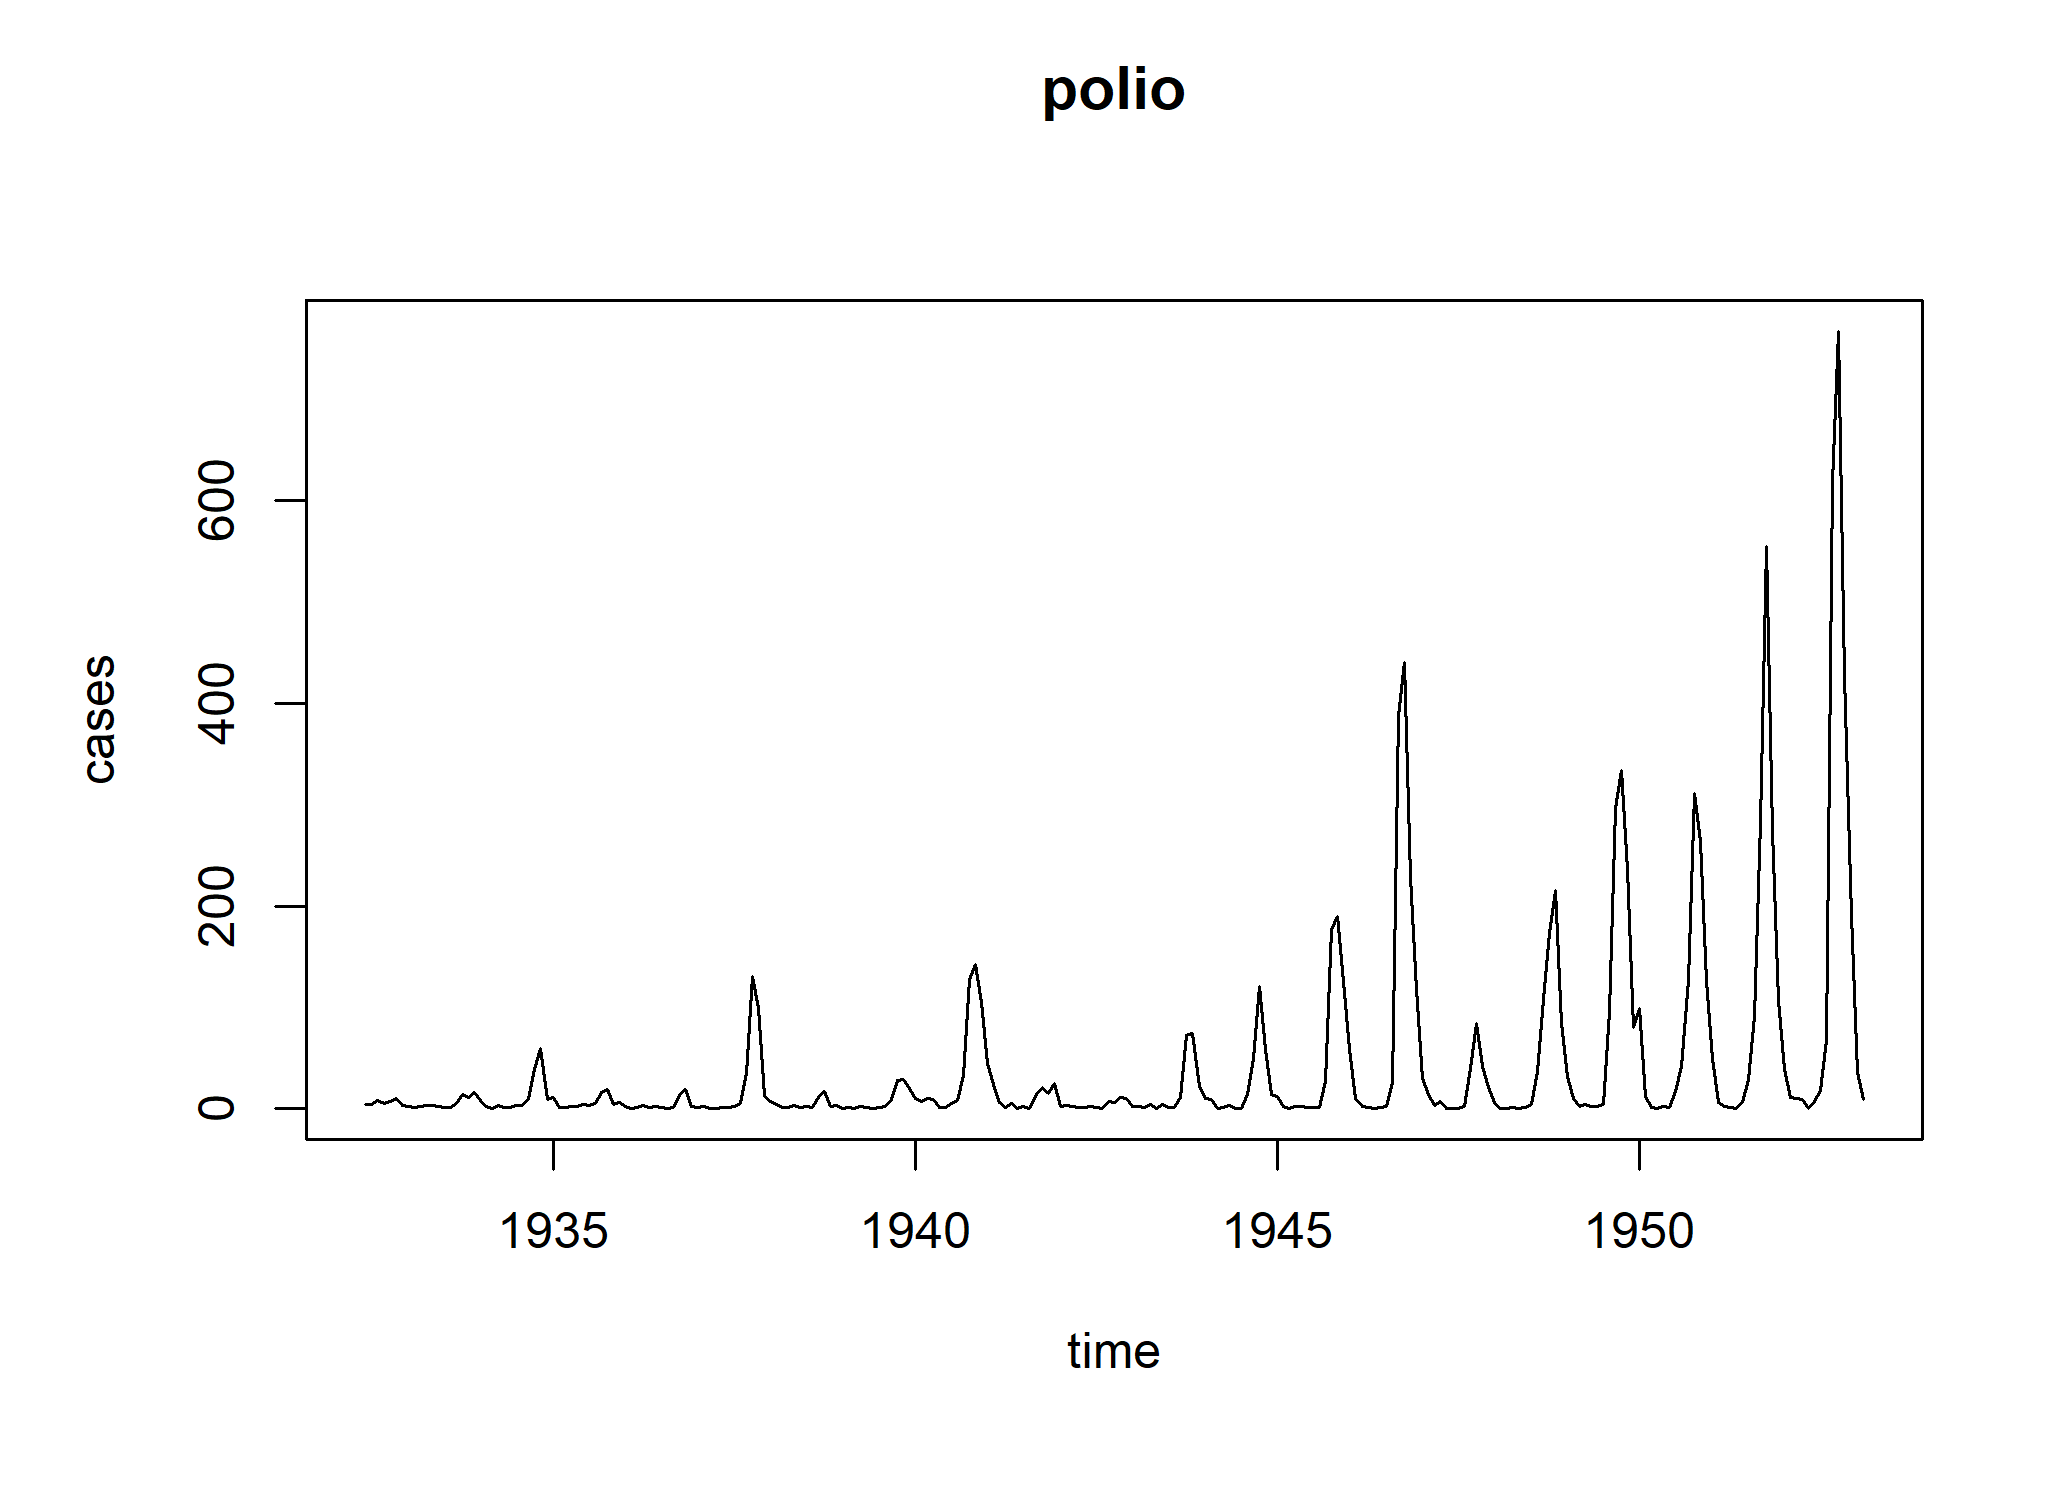
\includegraphics{figure/sp500-pomp-1} \end{center}

\begin{center}\rule{0.5\linewidth}{\linethickness}\end{center}

\begin{center}\rule{0.5\linewidth}{\linethickness}\end{center}

\subsection{Setting run levels to control computation
time}\label{setting-run-levels-to-control-computation-time}

\begin{itemize}
\item
  To develop and debug code, it is nice to have a version that runs
  extra quickly.
\item
  To facilitate switching quickly between versions of the document that
  have different run times, we set up \texttt{run\_level} options.
\item
  \texttt{run\_level=1} will set all the algorithmic parameters to the
  first column of values in the following code.
\item
  Here, \texttt{Np} is the number of particles (i.e., sequential Monte
  Carlo sample size), and \texttt{Nmif} is the number of iterations of
  the optimization procedure carried out below.
\item
  Empirically, \texttt{Np=5000} and \texttt{Nmif=200} are around the
  minimum required to get stable results with an error in the likelihood
  of order 1 log unit for this example; this is implemented by setting
  \texttt{run\_level=2}.
\item
  One can then ramp up to larger values for more refined computations,
  implemented here by \texttt{run\_level=3}.
\end{itemize}

\begin{Shaded}
\begin{Highlighting}[]
\NormalTok{run_level=}\DecValTok{3}
\NormalTok{polio_Np <-}\StringTok{          }\KeywordTok{c}\NormalTok{(}\DecValTok{100}\NormalTok{,}\FloatTok{5e3}\NormalTok{,}\FloatTok{1e4}\NormalTok{)}
\NormalTok{polio_Nmif <-}\StringTok{        }\KeywordTok{c}\NormalTok{(}\DecValTok{10}\NormalTok{, }\DecValTok{200}\NormalTok{,}\DecValTok{400}\NormalTok{)}
\NormalTok{polio_Nreps_eval <-}\StringTok{  }\KeywordTok{c}\NormalTok{(}\DecValTok{2}\NormalTok{,  }\DecValTok{10}\NormalTok{,  }\DecValTok{20}\NormalTok{)}
\NormalTok{polio_Nreps_local <-}\StringTok{ }\KeywordTok{c}\NormalTok{(}\DecValTok{10}\NormalTok{, }\DecValTok{20}\NormalTok{, }\DecValTok{40}\NormalTok{)}
\NormalTok{polio_Nreps_global <-}\KeywordTok{c}\NormalTok{(}\DecValTok{10}\NormalTok{, }\DecValTok{20}\NormalTok{, }\DecValTok{100}\NormalTok{)}
\NormalTok{polio_Nsim <-}\StringTok{        }\KeywordTok{c}\NormalTok{(}\DecValTok{50}\NormalTok{,}\DecValTok{100}\NormalTok{, }\DecValTok{500}\NormalTok{) }
\end{Highlighting}
\end{Shaded}

\begin{itemize}
\item
  Here, \texttt{run\_level} is coded differently from the previous case
  studies. It is functionally equivalent. Which way you prefer is up to
  you, but seeing different alternatives may help to clarify the goal of
  the code.
\item
  \texttt{run\_level} is a facility that is convenient for when you are
  editing the source code. It plays no fundamental role in the final
  results. If you are not editing the source code, or using the code as
  a template for developing your own analysis, it has no function.
\item
  When you edit a document with different \texttt{run\_level} options,
  you can debug your code by editing \texttt{run\_level=1}. Then, you
  can get preliminary assessment of whether your results are sensible
  with \texttt{run\_level=2} and get finalized results, with reduced
  Monte Carlo error, by editing \texttt{run\_level=3}.
\item
  In practice, you probably want \texttt{run\_level=1} to run in
  minutes, \texttt{run\_level=2} to run in tens of minutes, and
  \texttt{run\_level=3} to run in hours.
\item
  You can increase or decrease the numbers of particles, or the number
  of mif2 iterations, or the number of global searches carried out, to
  make sure this procedure is practical on your machine.
\item
  Appropriate values of the algorithmic parameters for each run-level
  are context dependent.
\end{itemize}

\begin{center}\rule{0.5\linewidth}{\linethickness}\end{center}

\subsubsection{Exercise: Choosing algorithmic
parameters}\label{exercise-choosing-algorithmic-parameters}

\begin{itemize}
\tightlist
\item
  Discuss how you choose the algorithmic parameters for each run level
  when building a new likelihood-based data analysis using
  \texttt{pfilter()} and \texttt{mif2()} in \textbf{pomp}.
\end{itemize}

\begin{center}\rule{0.5\linewidth}{\linethickness}\end{center}

\begin{center}\rule{0.5\linewidth}{\linethickness}\end{center}

\subsection{Likelihood evaluation at an estimated
MLE}\label{likelihood-evaluation-at-an-estimated-mle}

\begin{itemize}
\item
  Let's carry out a likelihood evaluation at the reported MLE.
\item
  Since most modern machines have multiple cores, it is convenient to do
  some parallelization to generate replicated calls to \texttt{pfilter}.
  Notice that the replications are averaged using the
  \texttt{logmeanexp} function.
\end{itemize}

\begin{Shaded}
\begin{Highlighting}[]
\KeywordTok{require}\NormalTok{(doParallel)}
\KeywordTok{registerDoParallel}\NormalTok{()}
\end{Highlighting}
\end{Shaded}

\begin{Shaded}
\begin{Highlighting}[]
\KeywordTok{stew}\NormalTok{(}\DataTypeTok{file=}\KeywordTok{sprintf}\NormalTok{(}\StringTok{"pf1-%d.rda"}\NormalTok{,run_level),\{}
\NormalTok{  t1 <-}\StringTok{ }\KeywordTok{system.time}\NormalTok{(}
\NormalTok{    pf1 <-}\StringTok{ }\KeywordTok{foreach}\NormalTok{(}\DataTypeTok{i=}\DecValTok{1}\OperatorTok{:}\DecValTok{20}\NormalTok{,}\DataTypeTok{.packages=}\StringTok{'pomp'}\NormalTok{,}
                   \DataTypeTok{.options.multicore=}\KeywordTok{list}\NormalTok{(}\DataTypeTok{set.seed=}\OtherTok{TRUE}\NormalTok{)) }\OperatorTok\StringTok{ }\KeywordTok{try}\NormalTok{(}
                     \KeywordTok{pfilter}\NormalTok{(polio,}\DataTypeTok{Np=}\NormalTok{polio_Np[run_level])}
\NormalTok{                   )}
\NormalTok{  )}
\NormalTok{\},}\DataTypeTok{seed=}\DecValTok{493536993}\NormalTok{,}\DataTypeTok{kind=}\StringTok{"L'Ecuyer"}\NormalTok{)}
\NormalTok{(L1 <-}\StringTok{ }\KeywordTok{logmeanexp}\NormalTok{(}\KeywordTok{sapply}\NormalTok{(pf1,logLik),}\DataTypeTok{se=}\OtherTok{TRUE}\NormalTok{))}
\end{Highlighting}
\end{Shaded}

\begin{verbatim}
##                        se 
## -794.5299165    0.1076427
\end{verbatim}

\begin{itemize}
\tightlist
\item
  In 5.7 seconds, we obtain an unbiased likelihood estimate of -794.53
  with a Monte standard error of 0.11.
\end{itemize}

\begin{center}\rule{0.5\linewidth}{\linethickness}\end{center}

\begin{center}\rule{0.5\linewidth}{\linethickness}\end{center}

\subsubsection{Comparison of our implementation with Martinez-Bakker et
al.
(2015)}\label{comparison-of-our-implementation-with-martinez-bakker15}

This setup has minor differences in notation, model construction and
code compared to Martinez-Bakker et al. (2015). The MLE reported for
these data by Martinez-Bakker et al. (2015) is -794.34 (with Monte Carlo
evaluation error of 0.18) which is similar to the log likelihood at the
MLE for our model (-794.53 with Monte Carlo evaluation error 0.11). This
suggests that the differences do not substantially improve or decrease
the fit of our model compared to Martinez-Bakker et al. (2015). When
different calculations match reasonably closely, it demonstrates some
reproducibility of both results.

\begin{center}\rule{0.5\linewidth}{\linethickness}\end{center}

\begin{center}\rule{0.5\linewidth}{\linethickness}\end{center}

\subsection{Simulation to investigate the fitted model: Local
persistence}\label{simulation-to-investigate-the-fitted-model-local-persistence}

The scientific purpose of fitting a model typically involves analyzing
properties of the fitted model, often investigated using simulation.
Following Martinez-Bakker et al. (2015), we are interested in how often
months with no reported cases (\(Y_n=0\)) correspond to months without
any local asymptomatic cases, defined for our continuous state model as
\(I^B_n+I^O_n<1/2\). For Wisconsin, using our model at the estimated
MLE, we compute as follows:

\begin{Shaded}
\begin{Highlighting}[]
\KeywordTok{stew}\NormalTok{(}\KeywordTok{sprintf}\NormalTok{(}\StringTok{"persistence-%d.rda"}\NormalTok{,run_level),\{}
\NormalTok{  t_sim <-}\StringTok{ }\KeywordTok{system.time}\NormalTok{(}
\NormalTok{    sim <-}\StringTok{ }\KeywordTok{foreach}\NormalTok{(}\DataTypeTok{i=}\DecValTok{1}\OperatorTok{:}\NormalTok{polio_Nsim[run_level],}\DataTypeTok{.packages=}\StringTok{'pomp'}\NormalTok{,}
                   \DataTypeTok{.options.multicore=}\KeywordTok{list}\NormalTok{(}\DataTypeTok{set.seed=}\OtherTok{TRUE}\NormalTok{)) }\OperatorTok\StringTok{ }
\StringTok{      }\KeywordTok{simulate}\NormalTok{(polio)}
\NormalTok{  )}
\NormalTok{\},}\DataTypeTok{seed=}\DecValTok{493536993}\NormalTok{,}\DataTypeTok{kind=}\StringTok{"L'Ecuyer"}\NormalTok{)}

\NormalTok{no_cases_data <-}\StringTok{ }\KeywordTok{sum}\NormalTok{(}\KeywordTok{obs}\NormalTok{(polio)}\OperatorTok{==}\DecValTok{0}\NormalTok{)}
\NormalTok{no_cases_sim <-}\StringTok{ }\KeywordTok{sum}\NormalTok{(}\KeywordTok{sapply}\NormalTok{(sim,obs)}\OperatorTok{==}\DecValTok{0}\NormalTok{)}\OperatorTok{/}\KeywordTok{length}\NormalTok{(sim)}
\NormalTok{fadeout1_sim <-}\StringTok{ }\KeywordTok{sum}\NormalTok{(}\KeywordTok{sapply}\NormalTok{(sim,}\ControlFlowTok{function}\NormalTok{(po)}\KeywordTok{states}\NormalTok{(po)[}\StringTok{"IB"}\NormalTok{,]}\OperatorTok{+}\KeywordTok{states}\NormalTok{(po)[}\StringTok{"IO"}\NormalTok{,]}\OperatorTok{<}\DecValTok{1}\NormalTok{))}\OperatorTok{/}\KeywordTok{length}\NormalTok{(sim)}
\NormalTok{fadeout100_sim <-}\StringTok{ }\KeywordTok{sum}\NormalTok{(}\KeywordTok{sapply}\NormalTok{(sim,}\ControlFlowTok{function}\NormalTok{(po)}\KeywordTok{states}\NormalTok{(po)[}\StringTok{"IB"}\NormalTok{,]}\OperatorTok{+}\KeywordTok{states}\NormalTok{(po)[}\StringTok{"IO"}\NormalTok{,]}\OperatorTok{<}\DecValTok{100}\NormalTok{))}\OperatorTok{/}\KeywordTok{length}\NormalTok{(sim)}
\NormalTok{imports_sim <-}\StringTok{ }\KeywordTok{coef}\NormalTok{(polio)[}\StringTok{"psi"}\NormalTok{]}\OperatorTok{*}\KeywordTok{mean}\NormalTok{(}\KeywordTok{sapply}\NormalTok{(sim,}\ControlFlowTok{function}\NormalTok{(po) }\KeywordTok{mean}\NormalTok{(}\KeywordTok{states}\NormalTok{(po)[}\StringTok{"SO"}\NormalTok{,]}\OperatorTok{+}\KeywordTok{states}\NormalTok{(po)[}\StringTok{"SB1"}\NormalTok{,]}\OperatorTok{+}\KeywordTok{states}\NormalTok{(po)[}\StringTok{"SB2"}\NormalTok{,]}\OperatorTok{+}\KeywordTok{states}\NormalTok{(po)[}\StringTok{"SB3"}\NormalTok{,]}\OperatorTok{+}\KeywordTok{states}\NormalTok{(po)[}\StringTok{"SB4"}\NormalTok{,]}\OperatorTok{+}\KeywordTok{states}\NormalTok{(po)[}\StringTok{"SB5"}\NormalTok{,]}\OperatorTok{+}\KeywordTok{states}\NormalTok{(po)[}\StringTok{"SB6"}\NormalTok{,])))}\OperatorTok{/}\DecValTok{12}
\end{Highlighting}
\end{Shaded}

\begin{itemize}
\item
  For the data, there were 26 months with no reported cases, in
  reasonable accordance with the mean of 37.6 for simulations from the
  fitted model. Months with no asyptomatic infections for the
  simulations were rare, on average 0.5 months per simulation. Months
  with fewer than 100 infections averaged 53.1 per simulation, which in
  the context of a reporting rate of 0.0124 can explain the absences of
  case reports. For this model, the mean monthly infections due to
  importations (more specifically, due to the term \(\psi\), whatever
  its biological interpretation) is 137.1. This does not give much
  opportunity for local elimination of poliovirus. One could profile
  over \(\psi\) to investigate how sensitive this conclusion is to
  values of \(\psi\) consistent with the data.
\item
  It is also good practice to look at simulations from the fitted model:
\end{itemize}

\begin{Shaded}
\begin{Highlighting}[]
\NormalTok{mle_simulation <-}\StringTok{ }\KeywordTok{simulate}\NormalTok{(polio,}\DataTypeTok{seed=}\DecValTok{127}\NormalTok{)}
\KeywordTok{plot}\NormalTok{(mle_simulation)}
\end{Highlighting}
\end{Shaded}

\begin{center}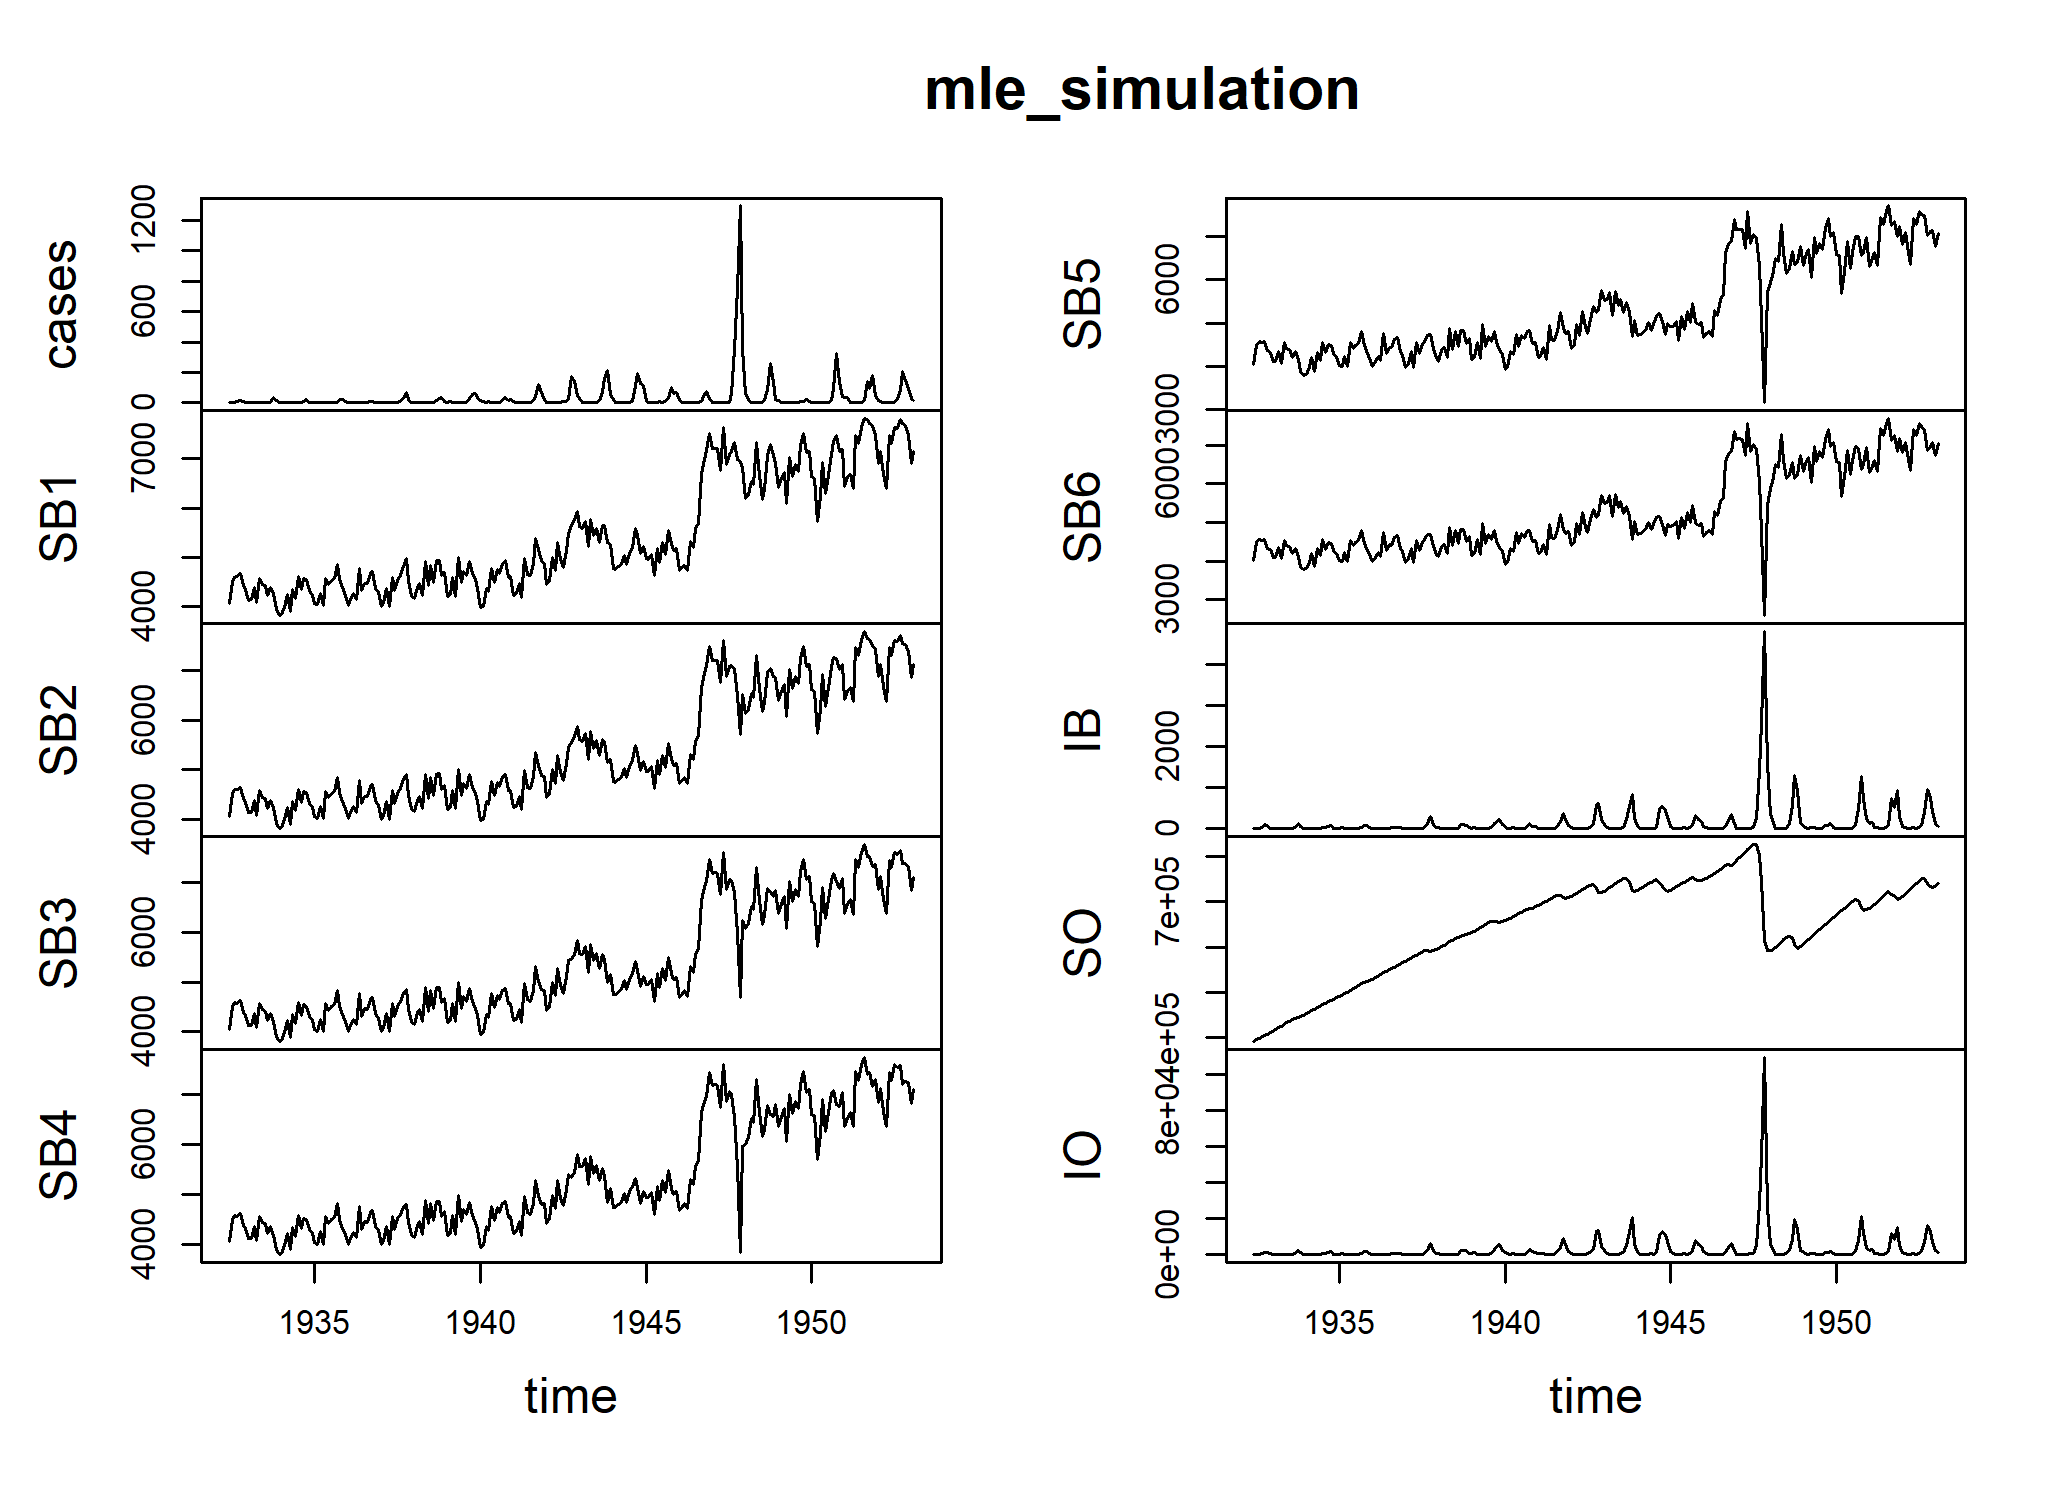
\includegraphics{figure/sp500-plot_simulated-1} \end{center}

\begin{itemize}
\item
  We see from this simulation that the fitted model can generate report
  histories that look qualitatively similar to the data. However, there
  are things to notice in the reconstructed latent states. Specifically,
  the pool of older susceptibles, \(S^O(t)\), is mostly increasing. The
  reduced case burden in the data in the time interval 1932--1945 is
  explained by a large initial recovered (\(R\)) population, which
  implies much higher levels of polio before 1932. There were large
  epidemics of polio in the USA early in the 20th century, so this is
  not implausible.
\item
  A liklihood profile over the parameter \(\tilde S^O_0\) could help to
  clarify to what extent this is a critical feature of how the model
  explains the data.
\end{itemize}

\begin{center}\rule{0.5\linewidth}{\linethickness}\end{center}

\begin{center}\rule{0.5\linewidth}{\linethickness}\end{center}

\subsection{Local likelihood
maximization}\label{local-likelihood-maximization}

\begin{itemize}
\tightlist
\item
  Let's see if we can improve on the previous MLE. We use the iterated
  filtering algorithm IF2 of Ionides et al. (2015), which uses a random
  walk in parameter space to approach the MLE. We set a constant random
  walk standard deviation for each of the regular parameters and a
  larger constant for each of the initial value parameters.
\end{itemize}

\begin{Shaded}
\begin{Highlighting}[]
\NormalTok{polio_rw.sd_rp <-}\StringTok{ }\FloatTok{0.02}
\NormalTok{polio_rw.sd_ivp <-}\StringTok{ }\FloatTok{0.2}
\NormalTok{polio_cooling.fraction.}\DecValTok{50}\NormalTok{ <-}\StringTok{ }\FloatTok{0.5}

\KeywordTok{stew}\NormalTok{(}\KeywordTok{sprintf}\NormalTok{(}\StringTok{"mif-%d.rda"}\NormalTok{,run_level),\{}
\NormalTok{  t2 <-}\StringTok{ }\KeywordTok{system.time}\NormalTok{(\{}
\NormalTok{    m2 <-}\StringTok{ }\KeywordTok{foreach}\NormalTok{(}\DataTypeTok{i=}\DecValTok{1}\OperatorTok{:}\NormalTok{polio_Nreps_local[run_level],}
                  \DataTypeTok{.packages=}\StringTok{'pomp'}\NormalTok{, }\DataTypeTok{.combine=}\NormalTok{c,}
                  \DataTypeTok{.options.multicore=}\KeywordTok{list}\NormalTok{(}\DataTypeTok{set.seed=}\OtherTok{TRUE}\NormalTok{)) }\OperatorTok\StringTok{ }\KeywordTok{try}\NormalTok{(}
                    \KeywordTok{mif2}\NormalTok{(polio,}
                         \DataTypeTok{Np=}\NormalTok{polio_Np[run_level],}
                         \DataTypeTok{Nmif=}\NormalTok{polio_Nmif[run_level],}
                         \DataTypeTok{cooling.type=}\StringTok{"geometric"}\NormalTok{,}
                         \DataTypeTok{cooling.fraction.50=}\NormalTok{polio_cooling.fraction.}\DecValTok{50}\NormalTok{,}
                         \DataTypeTok{transform=}\OtherTok{TRUE}\NormalTok{,}
                         \DataTypeTok{rw.sd=}\KeywordTok{rw.sd}\NormalTok{(}
                           \DataTypeTok{b1=}\NormalTok{polio_rw.sd_rp,}
                           \DataTypeTok{b2=}\NormalTok{polio_rw.sd_rp,}
                           \DataTypeTok{b3=}\NormalTok{polio_rw.sd_rp,}
                           \DataTypeTok{b4=}\NormalTok{polio_rw.sd_rp,}
                           \DataTypeTok{b5=}\NormalTok{polio_rw.sd_rp,}
                           \DataTypeTok{b6=}\NormalTok{polio_rw.sd_rp,}
                           \DataTypeTok{psi=}\NormalTok{polio_rw.sd_rp,}
                           \DataTypeTok{rho=}\NormalTok{polio_rw.sd_rp,}
                           \DataTypeTok{tau=}\NormalTok{polio_rw.sd_rp,}
                           \DataTypeTok{sigma_dem=}\NormalTok{polio_rw.sd_rp,}
                           \DataTypeTok{sigma_env=}\NormalTok{polio_rw.sd_rp,}
                           \DataTypeTok{IO_0=}\KeywordTok{ivp}\NormalTok{(polio_rw.sd_ivp),}
                           \DataTypeTok{SO_0=}\KeywordTok{ivp}\NormalTok{(polio_rw.sd_ivp)}
\NormalTok{                         )}
\NormalTok{                    )}
\NormalTok{                  )}
    
\NormalTok{    lik_m2 <-}\StringTok{ }\KeywordTok{foreach}\NormalTok{(}\DataTypeTok{i=}\DecValTok{1}\OperatorTok{:}\NormalTok{polio_Nreps_local[run_level],}\DataTypeTok{.packages=}\StringTok{'pomp'}\NormalTok{,}
                      \DataTypeTok{.combine=}\NormalTok{rbind,}\DataTypeTok{.options.multicore=}\KeywordTok{list}\NormalTok{(}\DataTypeTok{set.seed=}\OtherTok{TRUE}\NormalTok{)) }\OperatorTok\StringTok{ }
\StringTok{                      }\NormalTok{\{}
                        \KeywordTok{logmeanexp}\NormalTok{(}
                          \KeywordTok{replicate}\NormalTok{(polio_Nreps_eval[run_level],}
                                    \KeywordTok{logLik}\NormalTok{(}\KeywordTok{pfilter}\NormalTok{(polio,}\DataTypeTok{params=}\KeywordTok{coef}\NormalTok{(m2[[i]]),}\DataTypeTok{Np=}\NormalTok{polio_Np[run_level]))}
\NormalTok{                          ),}
                          \DataTypeTok{se=}\OtherTok{TRUE}\NormalTok{)}
\NormalTok{                      \}}
\NormalTok{  \})}
\NormalTok{\},}\DataTypeTok{seed=}\DecValTok{318817883}\NormalTok{,}\DataTypeTok{kind=}\StringTok{"L'Ecuyer"}\NormalTok{)}

\NormalTok{r2 <-}\StringTok{ }\KeywordTok{data.frame}\NormalTok{(}\DataTypeTok{logLik=}\NormalTok{lik_m2[,}\DecValTok{1}\NormalTok{],}\DataTypeTok{logLik_se=}\NormalTok{lik_m2[,}\DecValTok{2}\NormalTok{],}\KeywordTok{t}\NormalTok{(}\KeywordTok{sapply}\NormalTok{(m2,coef)))}
\ControlFlowTok{if}\NormalTok{ (run_level}\OperatorTok{>}\DecValTok{1}\NormalTok{) }
  \KeywordTok{write.table}\NormalTok{(r2,}\DataTypeTok{file=}\StringTok{"polio_params.csv"}\NormalTok{,}\DataTypeTok{append=}\OtherTok{TRUE}\NormalTok{,}\DataTypeTok{col.names=}\OtherTok{FALSE}\NormalTok{,}\DataTypeTok{row.names=}\OtherTok{FALSE}\NormalTok{)}
\KeywordTok{summary}\NormalTok{(r2}\OperatorTok{$}\NormalTok{logLik,}\DataTypeTok{digits=}\DecValTok{5}\NormalTok{)}
\end{Highlighting}
\end{Shaded}

\begin{verbatim}
##    Min. 1st Qu.  Median    Mean 3rd Qu.    Max. 
## -1026.7  -795.2  -795.0  -813.4  -794.9  -794.4
\end{verbatim}

\begin{itemize}
\tightlist
\item
  This investigation took 185.3 minutes. These repeated stochastic
  maximizations can also show us the geometry of the likelihood surface
  in a neighborhood of this point estimate:
\end{itemize}

\begin{Shaded}
\begin{Highlighting}[]
\KeywordTok{pairs}\NormalTok{(}\OperatorTok{~}\NormalTok{logLik}\OperatorTok{+}\NormalTok{psi}\OperatorTok{+}\NormalTok{rho}\OperatorTok{+}\NormalTok{tau}\OperatorTok{+}\NormalTok{sigma_dem}\OperatorTok{+}\NormalTok{sigma_env,}\DataTypeTok{data=}\KeywordTok{subset}\NormalTok{(r2,logLik}\OperatorTok{>}\KeywordTok{max}\NormalTok{(logLik)}\OperatorTok{-}\DecValTok{20}\NormalTok{))}
\end{Highlighting}
\end{Shaded}

\begin{center}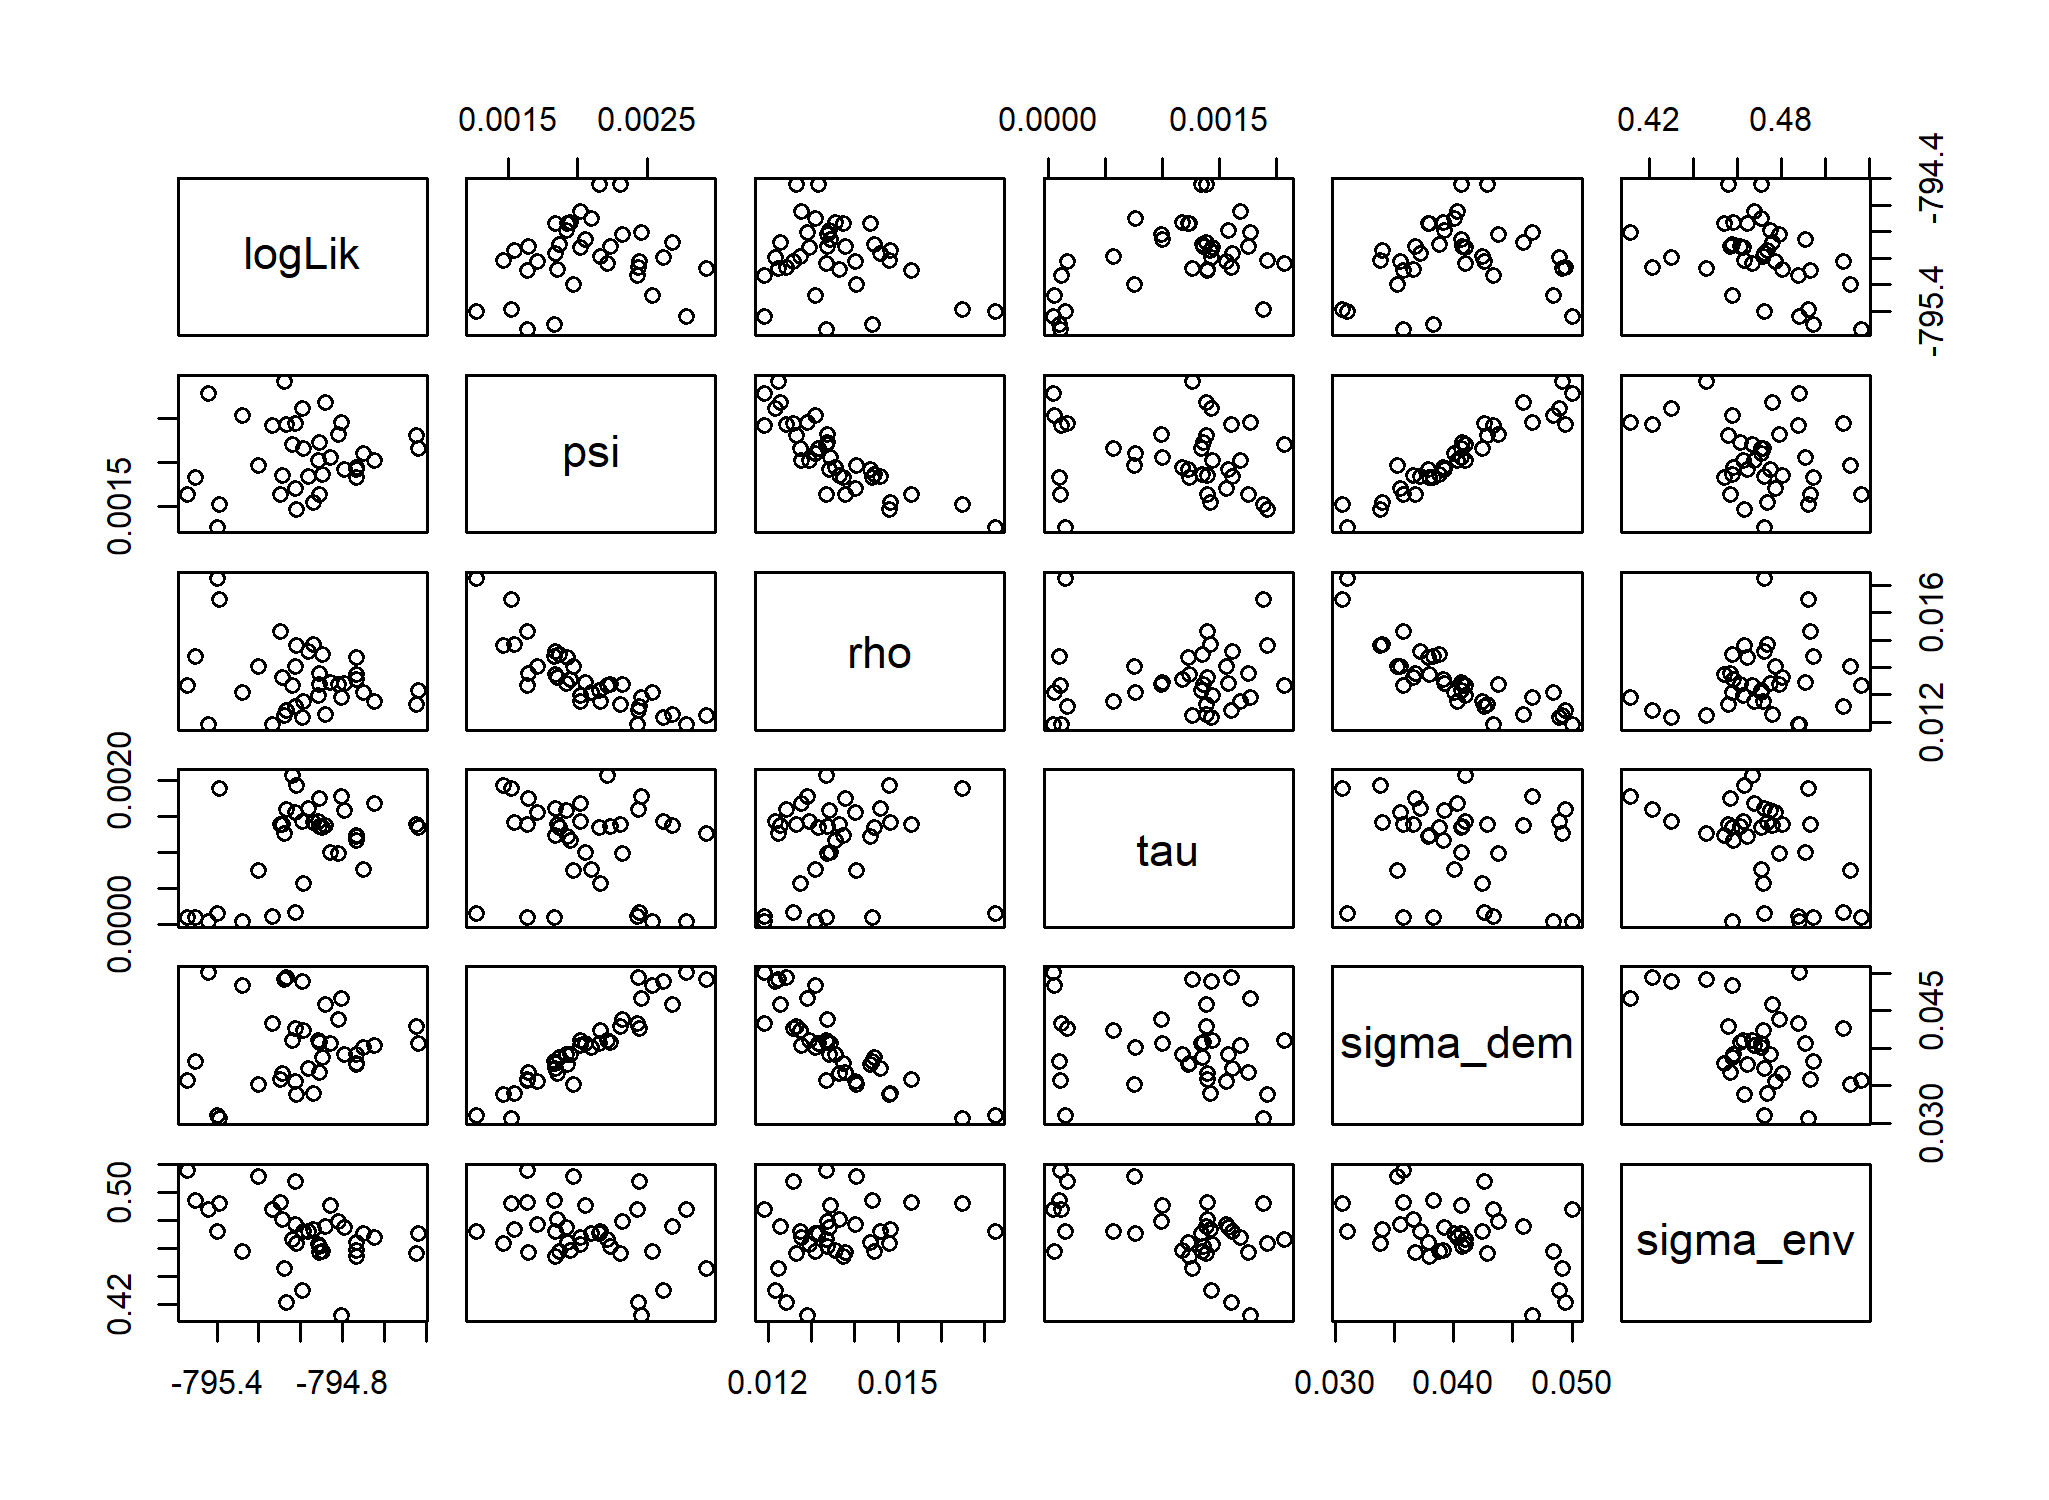
\includegraphics{figure/sp500-pairs-1} \end{center}

\begin{itemize}
\tightlist
\item
  We see strong tradeoffs between \(\psi\), \(\rho\) and
  \(\sigma_\mathrm{dem}\). By itself, in the absence of other
  assumptions, the pathogen immigration rate \(\psi\) is fairly weakly
  identified. However, the reporting rate \(\rho\) is essentially the
  fraction of poliovirus infections leading to acute flaccid paralysis,
  which is known to be around 1\%. This plot suggests that fixing an
  assumed value of \(\rho\) might lead to much more precise inference on
  \(\psi\); the rate of pathogen immigration presumably being important
  for understanding disease persistence. These hypotheses could be
  investigated more formally by construction of profile likelihood plots
  and likelihood ratio tests.
\end{itemize}

\begin{center}\rule{0.5\linewidth}{\linethickness}\end{center}

\begin{center}\rule{0.5\linewidth}{\linethickness}\end{center}

\subsection{Global likelihood
maximization}\label{global-likelihood-maximization}

When carrying out parameter estimation for dynamic systems, we need to
specify beginning values for both the dynamic system (in the state
space) and the parameters (in the parameter space). By convention, we
use \emph{initial values} for the initialization of the dynamic system
and \emph{starting values} for initialization of the parameter search.

Practical parameter estimation involves trying many starting values for
the parameters. One can specify a large box in parameter space that
contains all parameter vectors which seem remotely sensible. If an
estimation method gives stable conclusions with starting values drawn
randomly from this box, this gives some confidence that an adequate
global search has been carried out.

For our polio model, a box containing reasonable parameter values might
be

\begin{Shaded}
\begin{Highlighting}[]
\NormalTok{polio_box <-}\StringTok{ }\KeywordTok{rbind}\NormalTok{(}
  \DataTypeTok{b1=}\KeywordTok{c}\NormalTok{(}\OperatorTok{-}\DecValTok{2}\NormalTok{,}\DecValTok{8}\NormalTok{),}
  \DataTypeTok{b2=}\KeywordTok{c}\NormalTok{(}\OperatorTok{-}\DecValTok{2}\NormalTok{,}\DecValTok{8}\NormalTok{),}
  \DataTypeTok{b3=}\KeywordTok{c}\NormalTok{(}\OperatorTok{-}\DecValTok{2}\NormalTok{,}\DecValTok{8}\NormalTok{),}
  \DataTypeTok{b4=}\KeywordTok{c}\NormalTok{(}\OperatorTok{-}\DecValTok{2}\NormalTok{,}\DecValTok{8}\NormalTok{),}
  \DataTypeTok{b5=}\KeywordTok{c}\NormalTok{(}\OperatorTok{-}\DecValTok{2}\NormalTok{,}\DecValTok{8}\NormalTok{),}
  \DataTypeTok{b6=}\KeywordTok{c}\NormalTok{(}\OperatorTok{-}\DecValTok{2}\NormalTok{,}\DecValTok{8}\NormalTok{),}
  \DataTypeTok{psi=}\KeywordTok{c}\NormalTok{(}\DecValTok{0}\NormalTok{,}\FloatTok{0.1}\NormalTok{),}
  \DataTypeTok{rho=}\KeywordTok{c}\NormalTok{(}\DecValTok{0}\NormalTok{,}\FloatTok{0.1}\NormalTok{),}
  \DataTypeTok{tau=}\KeywordTok{c}\NormalTok{(}\DecValTok{0}\NormalTok{,}\FloatTok{0.1}\NormalTok{),}
  \DataTypeTok{sigma_dem=}\KeywordTok{c}\NormalTok{(}\DecValTok{0}\NormalTok{,}\FloatTok{0.5}\NormalTok{),}
  \DataTypeTok{sigma_env=}\KeywordTok{c}\NormalTok{(}\DecValTok{0}\NormalTok{,}\DecValTok{1}\NormalTok{),}
  \DataTypeTok{SO_0=}\KeywordTok{c}\NormalTok{(}\DecValTok{0}\NormalTok{,}\DecValTok{1}\NormalTok{),}
  \DataTypeTok{IO_0=}\KeywordTok{c}\NormalTok{(}\DecValTok{0}\NormalTok{,}\FloatTok{0.01}\NormalTok{)}
\NormalTok{)}
\end{Highlighting}
\end{Shaded}

We then carry out a search identical to the local one except for the
starting parameter values. This can be succinctly coded by calling
\texttt{mif2} on the previously constructed object,
\texttt{m2{[}{[}1{]}{]}}, with a reset starting value:

\begin{Shaded}
\begin{Highlighting}[]
\KeywordTok{stew}\NormalTok{(}\DataTypeTok{file=}\KeywordTok{sprintf}\NormalTok{(}\StringTok{"box_eval-%d.rda"}\NormalTok{,run_level),\{}
\NormalTok{  t3 <-}\StringTok{ }\KeywordTok{system.time}\NormalTok{(\{}
\NormalTok{    m3 <-}\StringTok{ }\KeywordTok{foreach}\NormalTok{(}\DataTypeTok{i=}\DecValTok{1}\OperatorTok{:}\NormalTok{polio_Nreps_global[run_level],}\DataTypeTok{.packages=}\StringTok{'pomp'}\NormalTok{,}\DataTypeTok{.combine=}\NormalTok{c,}
                  \DataTypeTok{.options.multicore=}\KeywordTok{list}\NormalTok{(}\DataTypeTok{set.seed=}\OtherTok{TRUE}\NormalTok{)) }\OperatorTok\StringTok{  }
\StringTok{      }\KeywordTok{mif2}\NormalTok{(}
\NormalTok{        m2[[}\DecValTok{1}\NormalTok{]],}
        \DataTypeTok{start=}\KeywordTok{c}\NormalTok{(}\KeywordTok{apply}\NormalTok{(polio_box,}\DecValTok{1}\NormalTok{,}\ControlFlowTok{function}\NormalTok{(x)}\KeywordTok{runif}\NormalTok{(}\DecValTok{1}\NormalTok{,x[}\DecValTok{1}\NormalTok{],x[}\DecValTok{2}\NormalTok{])),polio_fixed_params)}
\NormalTok{      )}
    
\NormalTok{    lik_m3 <-}\StringTok{ }\KeywordTok{foreach}\NormalTok{(}\DataTypeTok{i=}\DecValTok{1}\OperatorTok{:}\NormalTok{polio_Nreps_global[run_level],}\DataTypeTok{.packages=}\StringTok{'pomp'}\NormalTok{,}\DataTypeTok{.combine=}\NormalTok{rbind,}
                      \DataTypeTok{.options.multicore=}\KeywordTok{list}\NormalTok{(}\DataTypeTok{set.seed=}\OtherTok{TRUE}\NormalTok{)) }\OperatorTok\StringTok{ }\NormalTok{\{}
                        \KeywordTok{set.seed}\NormalTok{(}\DecValTok{87932}\OperatorTok{+}\NormalTok{i)}
                        \KeywordTok{logmeanexp}\NormalTok{(}
                          \KeywordTok{replicate}\NormalTok{(polio_Nreps_eval[run_level],}
                                    \KeywordTok{logLik}\NormalTok{(}\KeywordTok{pfilter}\NormalTok{(polio,}\DataTypeTok{params=}\KeywordTok{coef}\NormalTok{(m3[[i]]),}\DataTypeTok{Np=}\NormalTok{polio_Np[run_level]))}
\NormalTok{                          ), }
                          \DataTypeTok{se=}\OtherTok{TRUE}\NormalTok{)}
\NormalTok{                      \}}
\NormalTok{  \})}
\NormalTok{\},}\DataTypeTok{seed=}\DecValTok{290860873}\NormalTok{,}\DataTypeTok{kind=}\StringTok{"L'Ecuyer"}\NormalTok{)}


\NormalTok{r3 <-}\StringTok{ }\KeywordTok{data.frame}\NormalTok{(}\DataTypeTok{logLik=}\NormalTok{lik_m3[,}\DecValTok{1}\NormalTok{],}\DataTypeTok{logLik_se=}\NormalTok{lik_m3[,}\DecValTok{2}\NormalTok{],}\KeywordTok{t}\NormalTok{(}\KeywordTok{sapply}\NormalTok{(m3,coef)))}
\ControlFlowTok{if}\NormalTok{(run_level}\OperatorTok{>}\DecValTok{1}\NormalTok{) }\KeywordTok{write.table}\NormalTok{(r3,}\DataTypeTok{file=}\StringTok{"polio_params.csv"}\NormalTok{,}\DataTypeTok{append=}\OtherTok{TRUE}\NormalTok{,}\DataTypeTok{col.names=}\OtherTok{FALSE}\NormalTok{,}\DataTypeTok{row.names=}\OtherTok{FALSE}\NormalTok{)}
\KeywordTok{summary}\NormalTok{(r3}\OperatorTok{$}\NormalTok{logLik,}\DataTypeTok{digits=}\DecValTok{5}\NormalTok{)}
\end{Highlighting}
\end{Shaded}

\begin{verbatim}
##    Min. 1st Qu.  Median    Mean 3rd Qu.    Max. 
## -1012.5  -795.6  -795.1  -805.7  -794.9  -794.5
\end{verbatim}

\begin{itemize}
\item
  Evaluation of the best result of this search gives a likelihood of
  -794.5 with a standard error of 0.1. We see that optimization attempts
  from diverse remote starting points can approach our MLE, but do not
  exceed it. This gives us some reasonable confidence in our MLE.
\item
  Plotting these diverse parameter estimates can help to give a feel for
  the global geometry of the likelihood surface
\end{itemize}

\begin{Shaded}
\begin{Highlighting}[]
\KeywordTok{pairs}\NormalTok{(}\OperatorTok{~}\NormalTok{logLik}\OperatorTok{+}\NormalTok{psi}\OperatorTok{+}\NormalTok{rho}\OperatorTok{+}\NormalTok{tau}\OperatorTok{+}\NormalTok{sigma_dem}\OperatorTok{+}\NormalTok{sigma_env,}\DataTypeTok{data=}\KeywordTok{subset}\NormalTok{(r3,logLik}\OperatorTok{>}\KeywordTok{max}\NormalTok{(logLik)}\OperatorTok{-}\DecValTok{20}\NormalTok{))}
\end{Highlighting}
\end{Shaded}

\begin{center}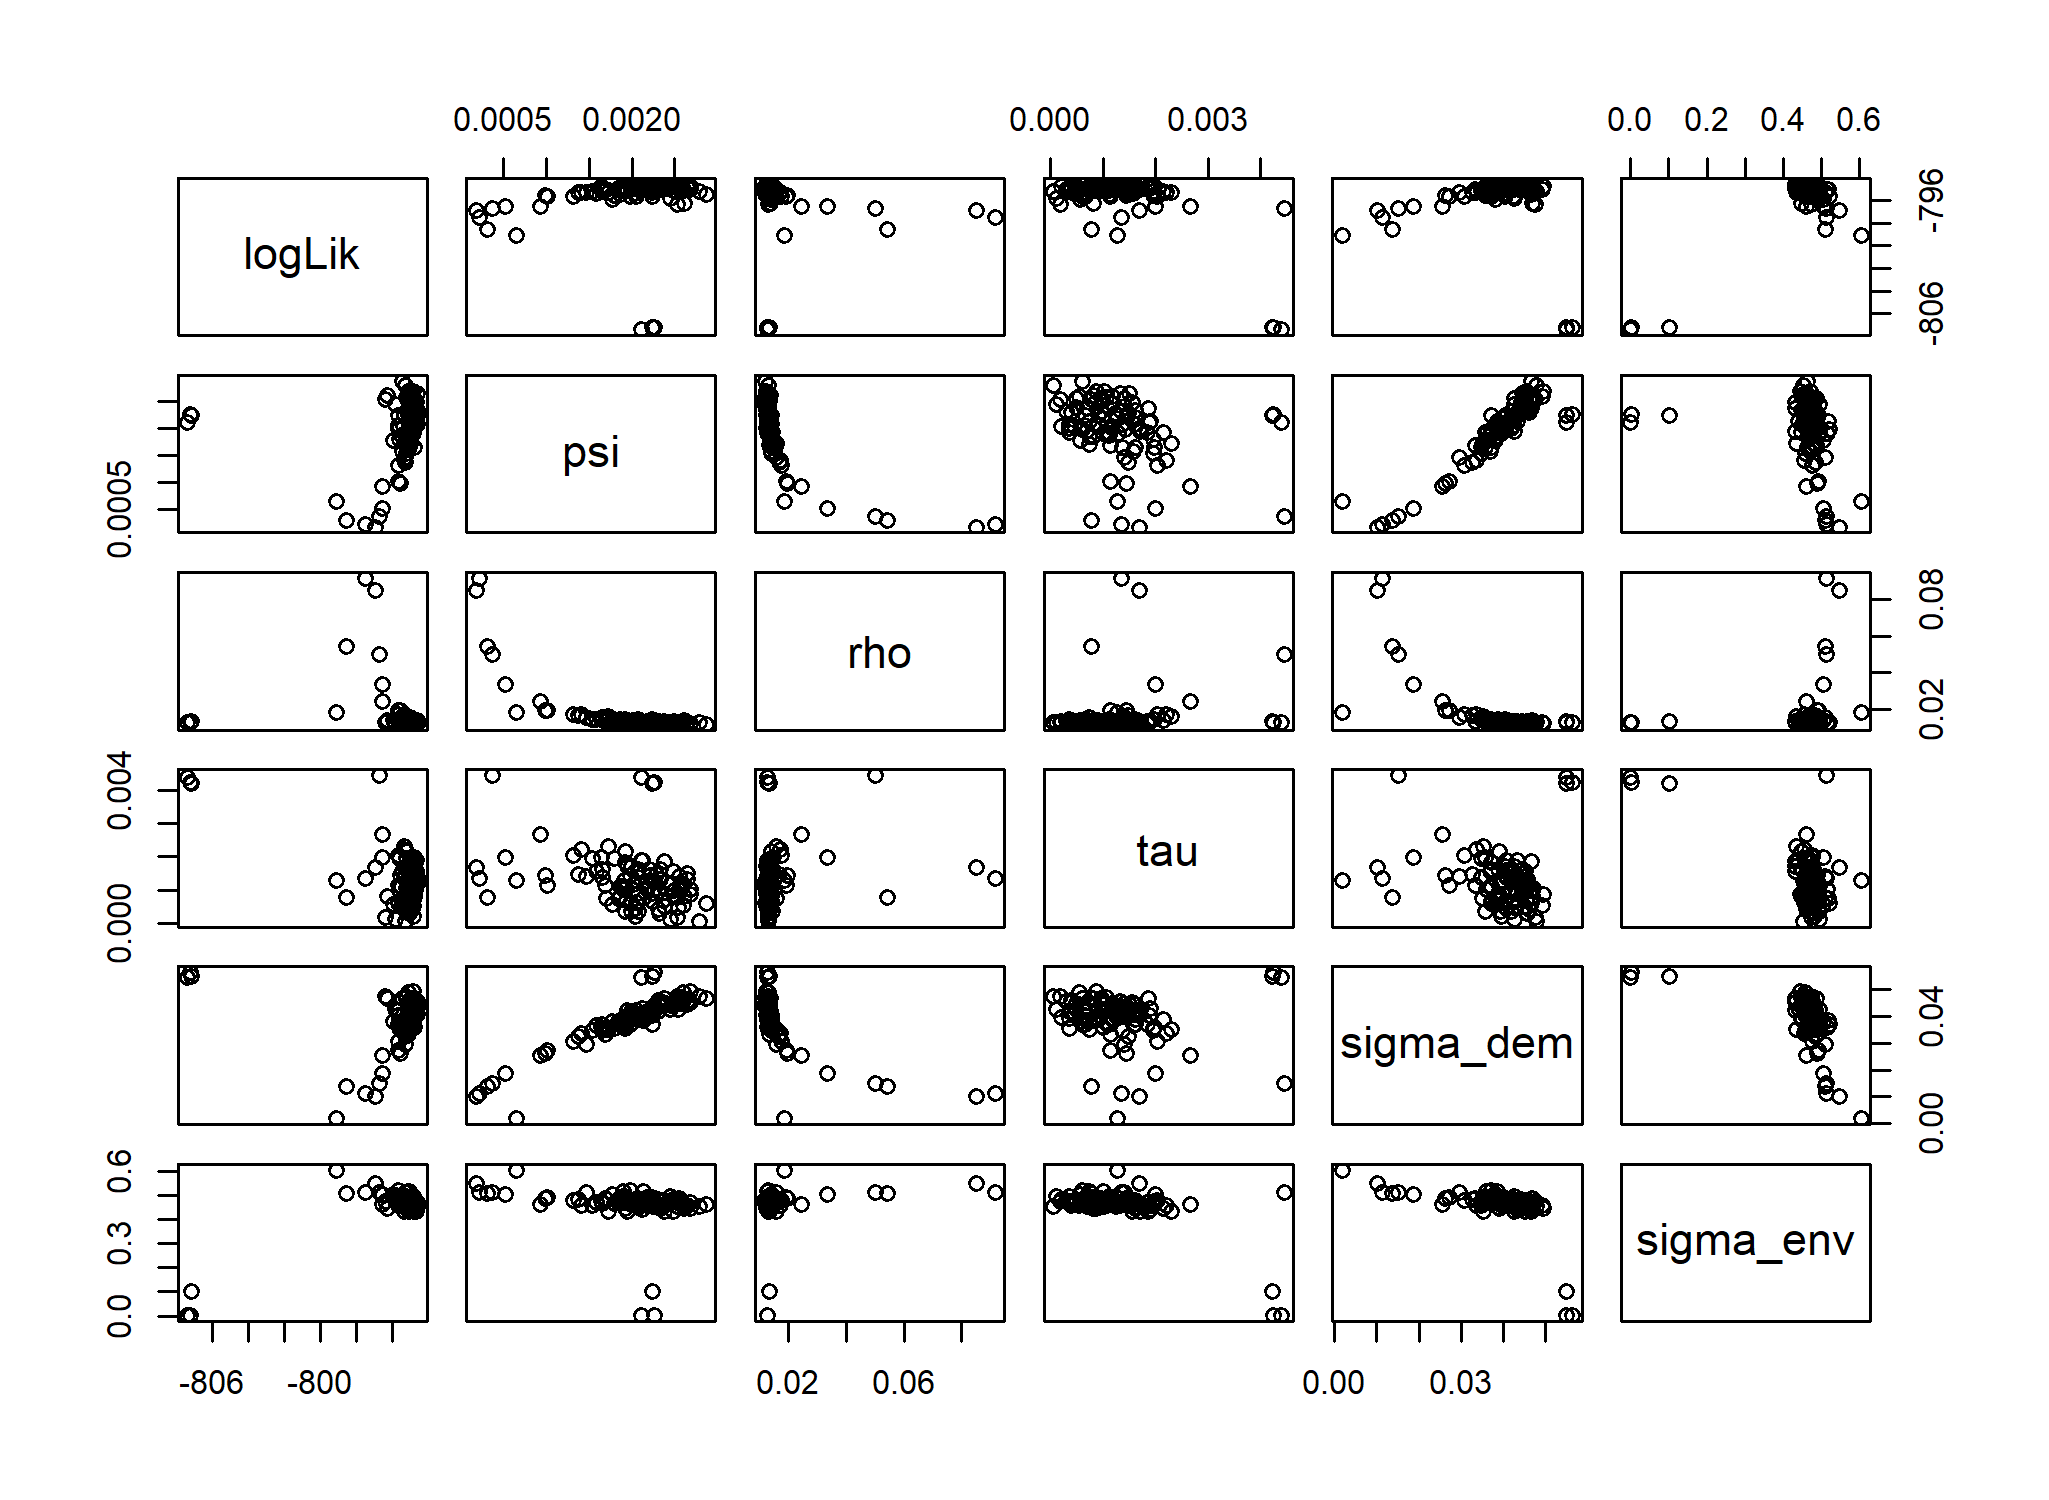
\includegraphics{figure/sp500-pairs_global-1} \end{center}

\begin{itemize}
\tightlist
\item
  To understand these global searches, many of which may correspond to
  parameter values having no meaningful scientific interpretation, it is
  helpful to put the log likelihoods in the context of some
  non-mechanistic benchmarks.
\end{itemize}

\subsubsection{Benchmark likelihoods for non-mechanistic
models}\label{benchmark-likelihoods-for-non-mechanistic-models}

\begin{itemize}
\tightlist
\item
  The most basic statistical model for data is independent, identically
  distributed (IID). Picking a negative binomial model,
\end{itemize}

\begin{Shaded}
\begin{Highlighting}[]
\NormalTok{nb_lik <-}\StringTok{ }\ControlFlowTok{function}\NormalTok{(theta) }\OperatorTok{-}\KeywordTok{sum}\NormalTok{(}\KeywordTok{dnbinom}\NormalTok{(}\KeywordTok{as.vector}\NormalTok{(}\KeywordTok{obs}\NormalTok{(polio)),}\DataTypeTok{size=}\KeywordTok{exp}\NormalTok{(theta[}\DecValTok{1}\NormalTok{]),}\DataTypeTok{prob=}\KeywordTok{exp}\NormalTok{(theta[}\DecValTok{2}\NormalTok{]),}\DataTypeTok{log=}\OtherTok{TRUE}\NormalTok{))}
\NormalTok{nb_mle <-}\StringTok{ }\KeywordTok{optim}\NormalTok{(}\KeywordTok{c}\NormalTok{(}\DecValTok{0}\NormalTok{,}\OperatorTok{-}\DecValTok{5}\NormalTok{),nb_lik)}
\OperatorTok{-}\NormalTok{nb_mle}\OperatorTok{$}\NormalTok{value}
\end{Highlighting}
\end{Shaded}

\begin{verbatim}
## [1] -1036.227
\end{verbatim}

\begin{itemize}
\item
  We see that a model with likelihood below -1036.2 is unreasonable.
  This explains a cutoff around this value in the global searches: in
  these cases, the model is finding essentially IID explanations for the
  data.
\item
  Linear, Gaussian auto-regressive moving-average (ARMA) models provide
  non-mechansitic fits to the data including flexible dependence
  relationships. We fit to \(\log(y_n^*+1)\) and correct the likelihood
  back to the scale appropriate for the untransformed data:
\end{itemize}

\begin{Shaded}
\begin{Highlighting}[]
\NormalTok{log_y <-}\StringTok{ }\KeywordTok{log}\NormalTok{(}\KeywordTok{as.vector}\NormalTok{(}\KeywordTok{obs}\NormalTok{(polio))}\OperatorTok{+}\DecValTok{1}\NormalTok{)}
\NormalTok{arma_fit <-}\StringTok{ }\KeywordTok{arima}\NormalTok{(log_y,}\DataTypeTok{order=}\KeywordTok{c}\NormalTok{(}\DecValTok{2}\NormalTok{,}\DecValTok{0}\NormalTok{,}\DecValTok{2}\NormalTok{),}\DataTypeTok{seasonal=}\KeywordTok{list}\NormalTok{(}\DataTypeTok{order=}\KeywordTok{c}\NormalTok{(}\DecValTok{1}\NormalTok{,}\DecValTok{0}\NormalTok{,}\DecValTok{1}\NormalTok{),}\DataTypeTok{period=}\DecValTok{12}\NormalTok{))}
\NormalTok{arma_fit}\OperatorTok{$}\NormalTok{loglik}\OperatorTok{-}\KeywordTok{sum}\NormalTok{(log_y)}
\end{Highlighting}
\end{Shaded}

\begin{verbatim}
## [1] -822.0827
\end{verbatim}

\begin{itemize}
\tightlist
\item
  This 7-parameter model, which knows nothing of susceptible depletion,
  attains a likelihood of -822.1. Although our goal is not to beat
  non-mechanstic models, it is comforting that we're competitive with
  them.
\end{itemize}

\begin{center}\rule{0.5\linewidth}{\linethickness}\end{center}

\begin{center}\rule{0.5\linewidth}{\linethickness}\end{center}

\subsubsection{Mining previous investigations of the
likelihood}\label{mining-previous-investigations-of-the-likelihood}

\begin{itemize}
\tightlist
\item
  Saving the results of previous searches, with likelihoods that have
  been repeatedly evaluated by particle filters, gives a resource for
  building up knowledge about the likelihood surface. Above, we have
  added our new results to the file \texttt{polio\_params.csv}, which we
  now investigate.
\end{itemize}

\begin{Shaded}
\begin{Highlighting}[]
\NormalTok{polio_params <-}\StringTok{ }\KeywordTok{read.table}\NormalTok{(}\StringTok{"polio_params.csv"}\NormalTok{,}\DataTypeTok{row.names=}\OtherTok{NULL}\NormalTok{,}\DataTypeTok{header=}\OtherTok{TRUE}\NormalTok{)}
\KeywordTok{pairs}\NormalTok{(}\OperatorTok{~}\NormalTok{logLik}\OperatorTok{+}\NormalTok{psi}\OperatorTok{+}\NormalTok{rho}\OperatorTok{+}\NormalTok{tau}\OperatorTok{+}\NormalTok{sigma_dem}\OperatorTok{+}\NormalTok{sigma_env,}\DataTypeTok{data=}\KeywordTok{subset}\NormalTok{(polio_params,logLik}\OperatorTok{>}\KeywordTok{max}\NormalTok{(logLik)}\OperatorTok{-}\DecValTok{20}\NormalTok{))}
\end{Highlighting}
\end{Shaded}

\begin{center}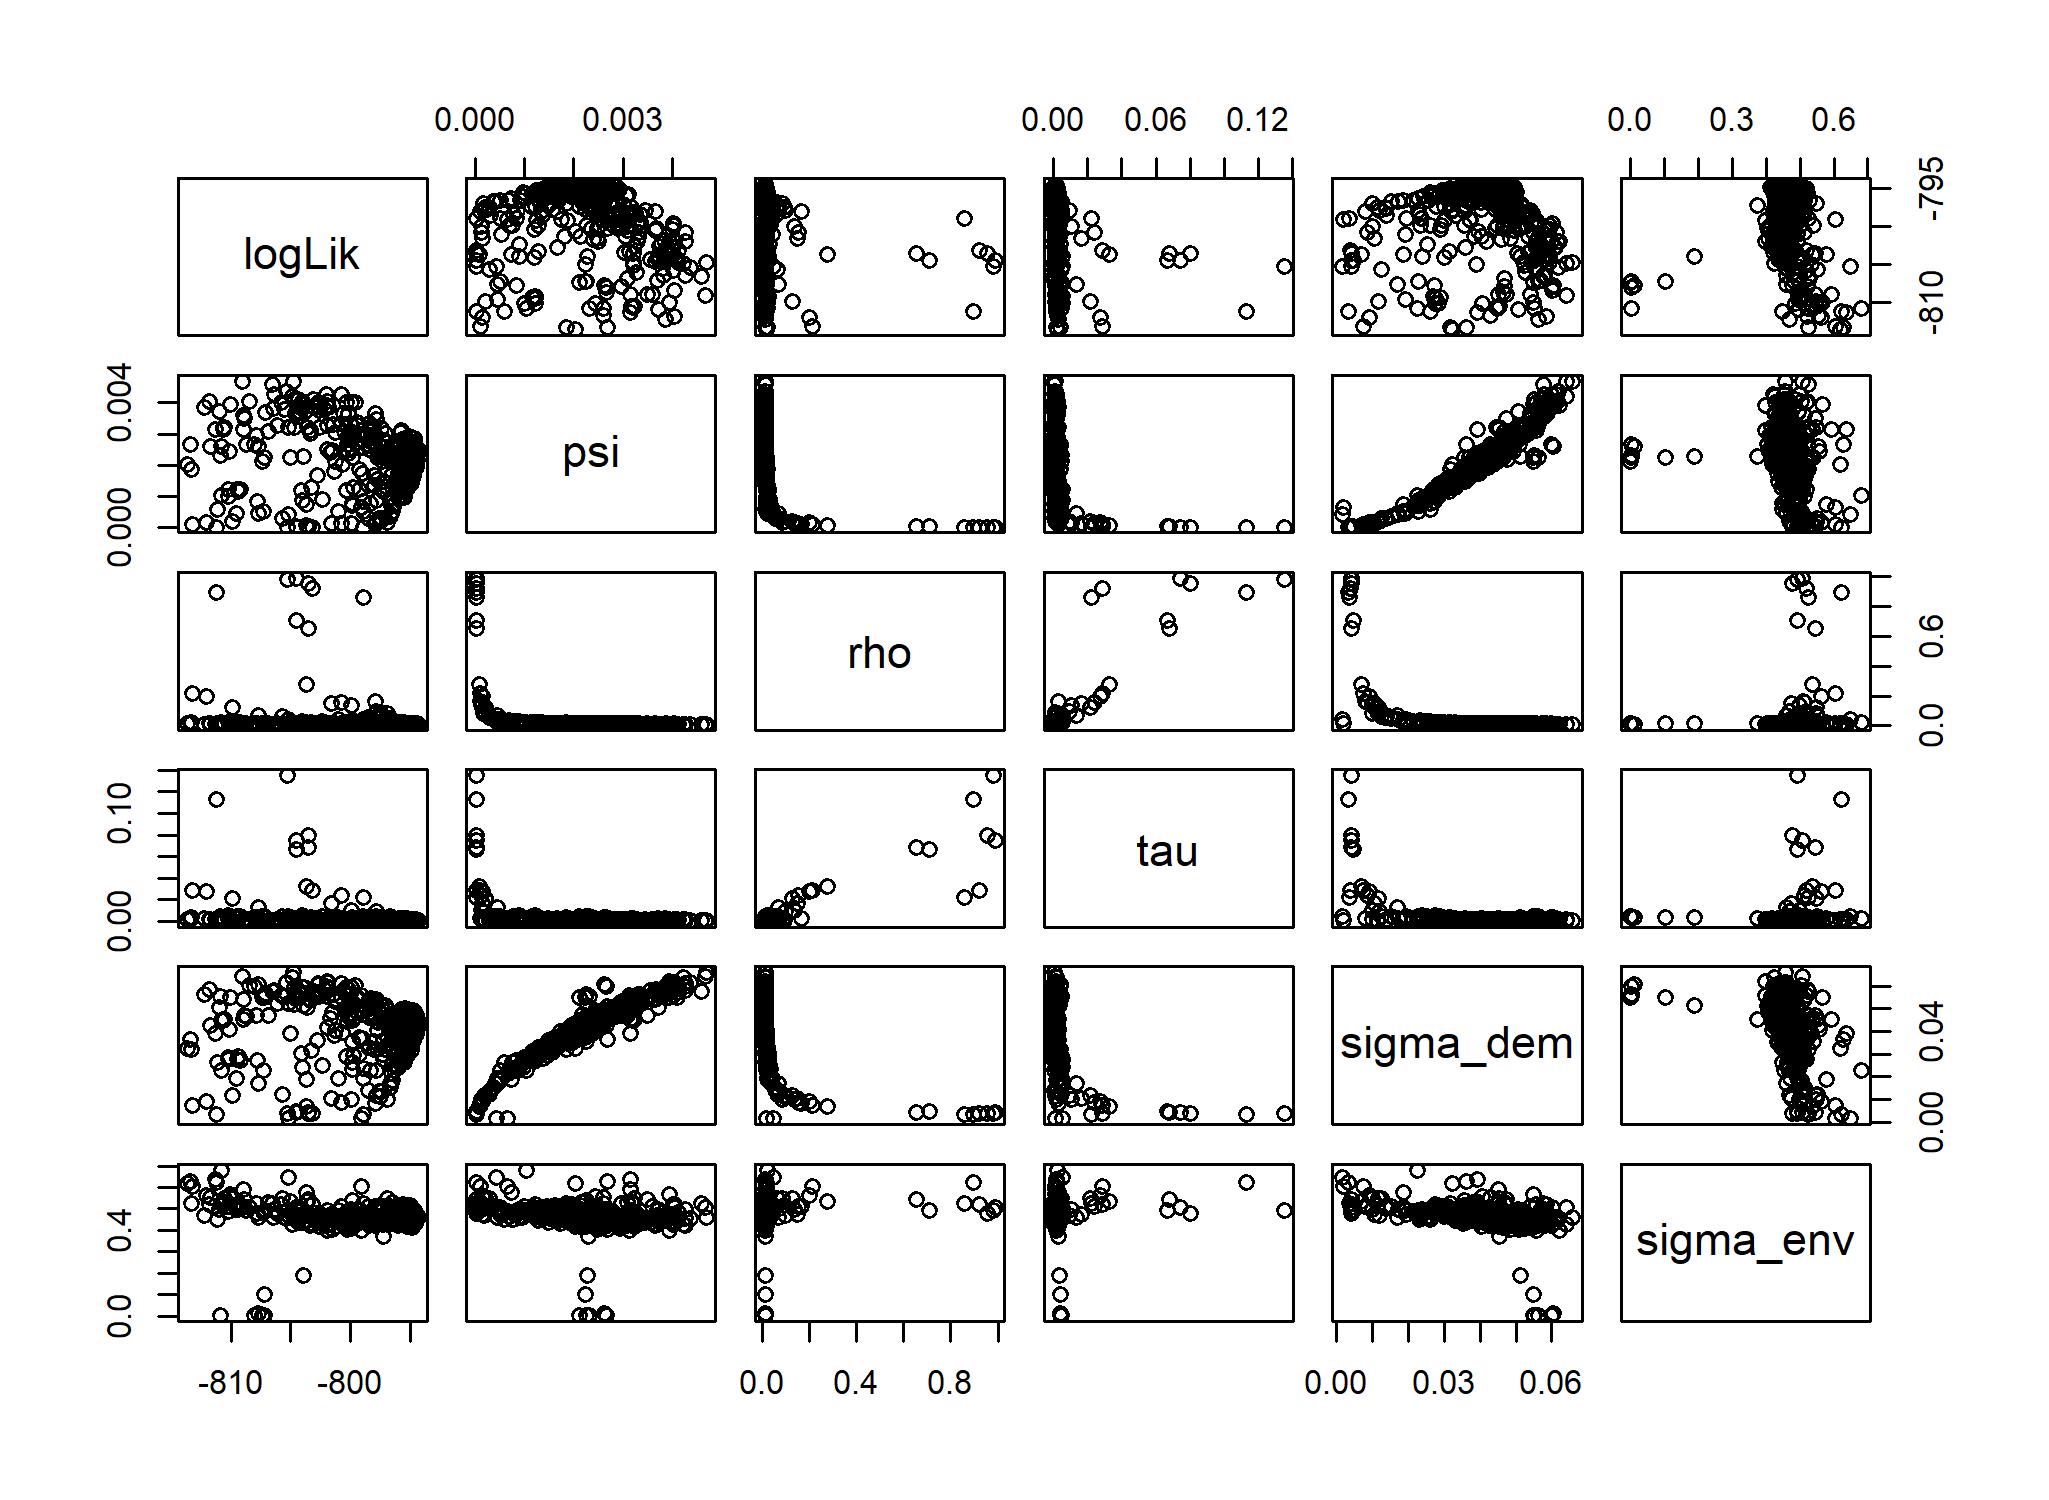
\includegraphics{figure/sp500-param_file-1} \end{center}

\begin{itemize}
\tightlist
\item
  Here, we see that the most successful searches have always led to
  models with reporting rate around 1\%. This impression can be
  reinforced by looking at results from the global searches:
\end{itemize}

\begin{Shaded}
\begin{Highlighting}[]
\KeywordTok{plot}\NormalTok{(logLik}\OperatorTok{~}\NormalTok{rho,}\DataTypeTok{data=}\KeywordTok{subset}\NormalTok{(r3,logLik}\OperatorTok{>}\KeywordTok{max}\NormalTok{(r3}\OperatorTok{$}\NormalTok{logLik)}\OperatorTok{-}\DecValTok{10}\NormalTok{),}\DataTypeTok{log=}\StringTok{"x"}\NormalTok{)}
\end{Highlighting}
\end{Shaded}

\begin{center}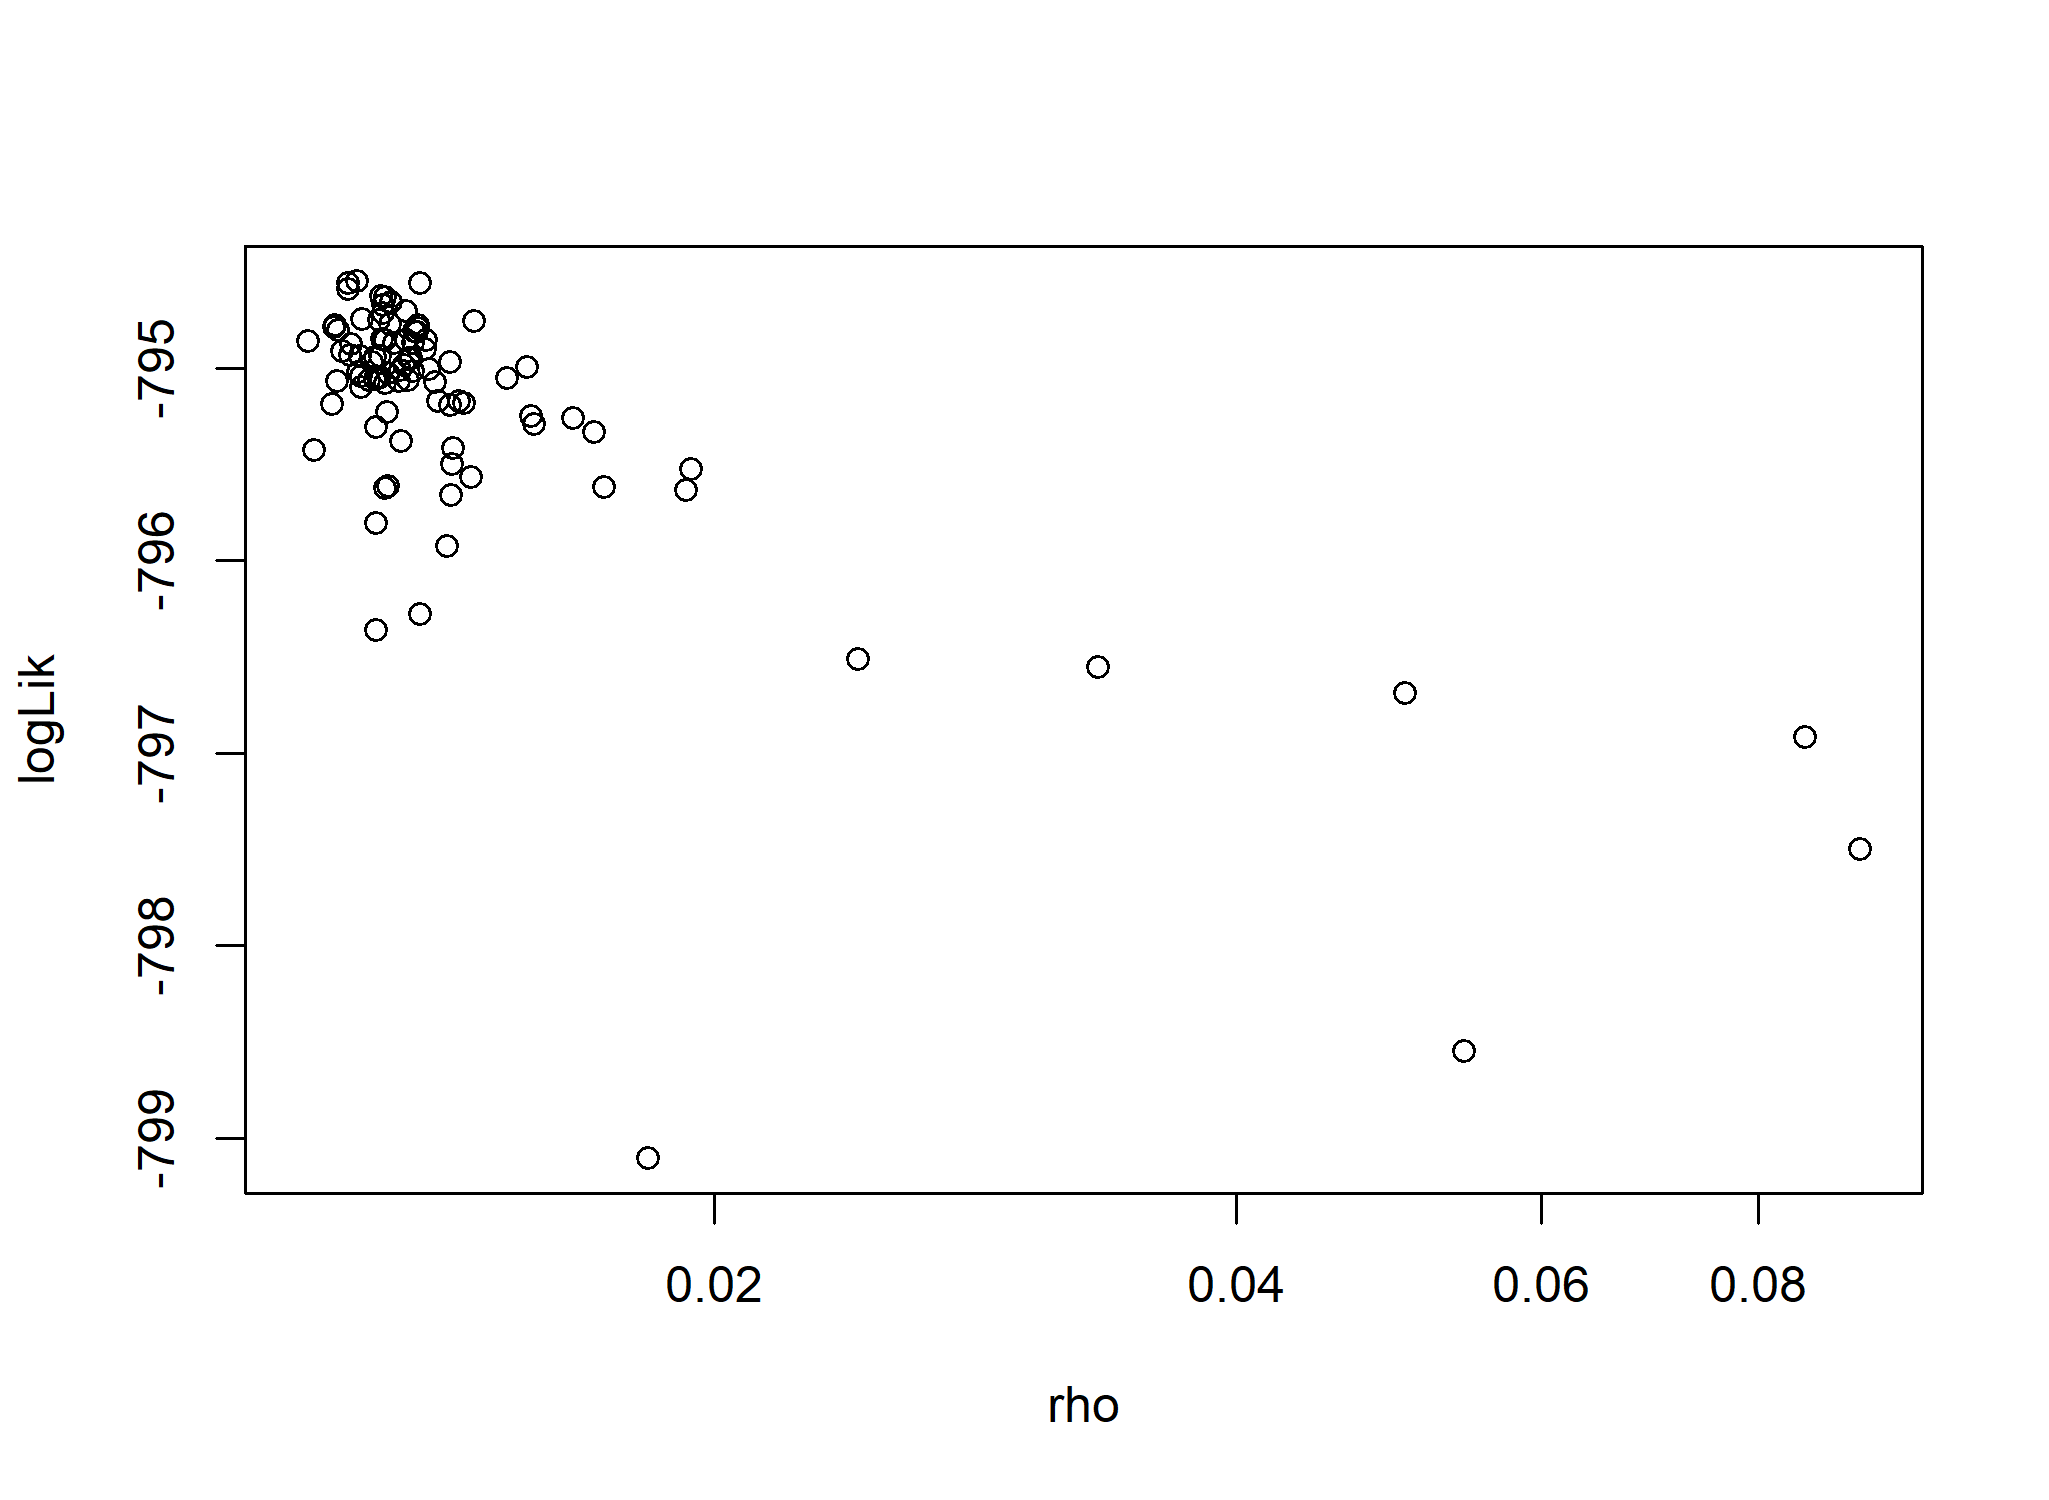
\includegraphics{figure/sp500-global_rho-1} \end{center}

\begin{itemize}
\tightlist
\item
  We see that reporting rates close to 1\% seem to provide a small but
  clear (several units of log likelihood) advantage in explaining the
  data. These are the reporting rates for which depletion of
  susceptibles can help to explain the dynamics.
\end{itemize}

\begin{center}\rule{0.5\linewidth}{\linethickness}\end{center}

\begin{center}\rule{0.5\linewidth}{\linethickness}\end{center}

\subsection{Exercises}\label{exercises}

\subsubsection{Exercise: Initial values}\label{exercise-initial-values}

When carrying out parameter estimation for dynamic systems, we need to
specify beginning values for both the dynamic system (in the state
space) and the parameters (in the parameter space). By convention, we
use \emph{initial values} for the initialization of the dynamic system
and \emph{starting values} for initialization of the parameter search.

Discuss issues in specifying and inferring initial conditions, with
particular reference to this polio example.

Suggest a possible improvement in the treatment of initial conditions
here, code it up and make some preliminary assessment of its
effectiveness. How will you decide if it is a substantial improvement?

\begin{center}\rule{0.5\linewidth}{\linethickness}\end{center}

\begin{center}\rule{0.5\linewidth}{\linethickness}\end{center}

\subsubsection{Exercise: Parameter estimation using randomized starting
values.}\label{exercise-parameter-estimation-using-randomized-starting-values.}

Comment on the computations above, for parameter estimation using
randomized starting values. Propose and try out at least one
modification of the procedure. How could one make a formal statement
quantifying the error of the optimization procedure?

\begin{center}\rule{0.5\linewidth}{\linethickness}\end{center}

\begin{center}\rule{0.5\linewidth}{\linethickness}\end{center}

\subsubsection{Exercise: Demography and discrete
time}\label{exercise-demography-and-discrete-time}

\begin{itemize}
\tightlist
\item
  It can be surprisingly hard to include birth, death, immigration,
  emmigration and aging into a disease model in satisfactory ways.
  Consider the strengths and weaknesses of the analysis presented. For
  example, how does it compare to a continuous-time model? In an
  imperfect world, it is nice to check the extent to which the
  conclusions are insensitive to alternative modeling decisions. If you
  have some ideas to change the treatmentof demography (or an other
  aspect of the model) you could have a go at coding it up to see if it
  makes a difference.
\end{itemize}

\begin{center}\rule{0.5\linewidth}{\linethickness}\end{center}

\begin{center}\rule{0.5\linewidth}{\linethickness}\end{center}

\subsubsection{Technical exercise: Diagnosing filtering and maximization
convergence}\label{technical-exercise-diagnosing-filtering-and-maximization-convergence}

Are there outliers in the data (i.e., observations that do not fit well
with our model)? Are we using unnecessarily large amounts of computer
time to get our results? Are there indications that we would should run
our computations for longer? Or maybe with different choices of
algorithmic settings?

In particular, \texttt{cooling.fraction.50} gives the fraction by which
the random walk standard deviation is decreased (``cooled'') in 50
iterations. If \texttt{cooling.fraction.50} is too small, the search
will ``freeze'' too soon, evidenced by flat parallel lines in the
convergence diagnostics. If \texttt{cooling.fraction.50} is too large,
the researcher may run of of time, patience or computing budget (or all
three) before the parameter trajectories approach an MLE.

Interpret the diagnostic plots below. Carry out some numerical
experiments to test your interpretations.

One could look at filtering diagnostics at the MLE, for example,
\texttt{plot(pf1{[}{[}1{]}{]})} but the diagnostic plots for iterated
filtering include filtering diagnostics for the last iteration anyhow,
so let's just consider the \texttt{mif} diagnostic plot. Looking at
several simultaneously permits assessment of Monte Carlo variability.
\texttt{plot} applied to a \texttt{mifList} object does this: here,
\texttt{m3} is of class \texttt{mifList} since that is the class
resulting from concatenation of \texttt{mif2d.pomp} objects using
\texttt{c()}:

\begin{Shaded}
\begin{Highlighting}[]
\KeywordTok{class}\NormalTok{(m3)}
\end{Highlighting}
\end{Shaded}

\begin{verbatim}
## [1] "mif2List"
## attr(,"package")
## [1] "pomp"
\end{verbatim}

\begin{Shaded}
\begin{Highlighting}[]
\KeywordTok{class}\NormalTok{(m3[[}\DecValTok{1}\NormalTok{]])}
\end{Highlighting}
\end{Shaded}

\begin{verbatim}
## [1] "mif2d.pomp"
## attr(,"package")
## [1] "pomp"
\end{verbatim}

\begin{Shaded}
\begin{Highlighting}[]
\KeywordTok{plot}\NormalTok{(m3[r3}\OperatorTok{$}\NormalTok{logLik}\OperatorTok{>}\KeywordTok{max}\NormalTok{(r3}\OperatorTok{$}\NormalTok{logLik)}\OperatorTok{-}\DecValTok{10}\NormalTok{])}
\end{Highlighting}
\end{Shaded}

\begin{center}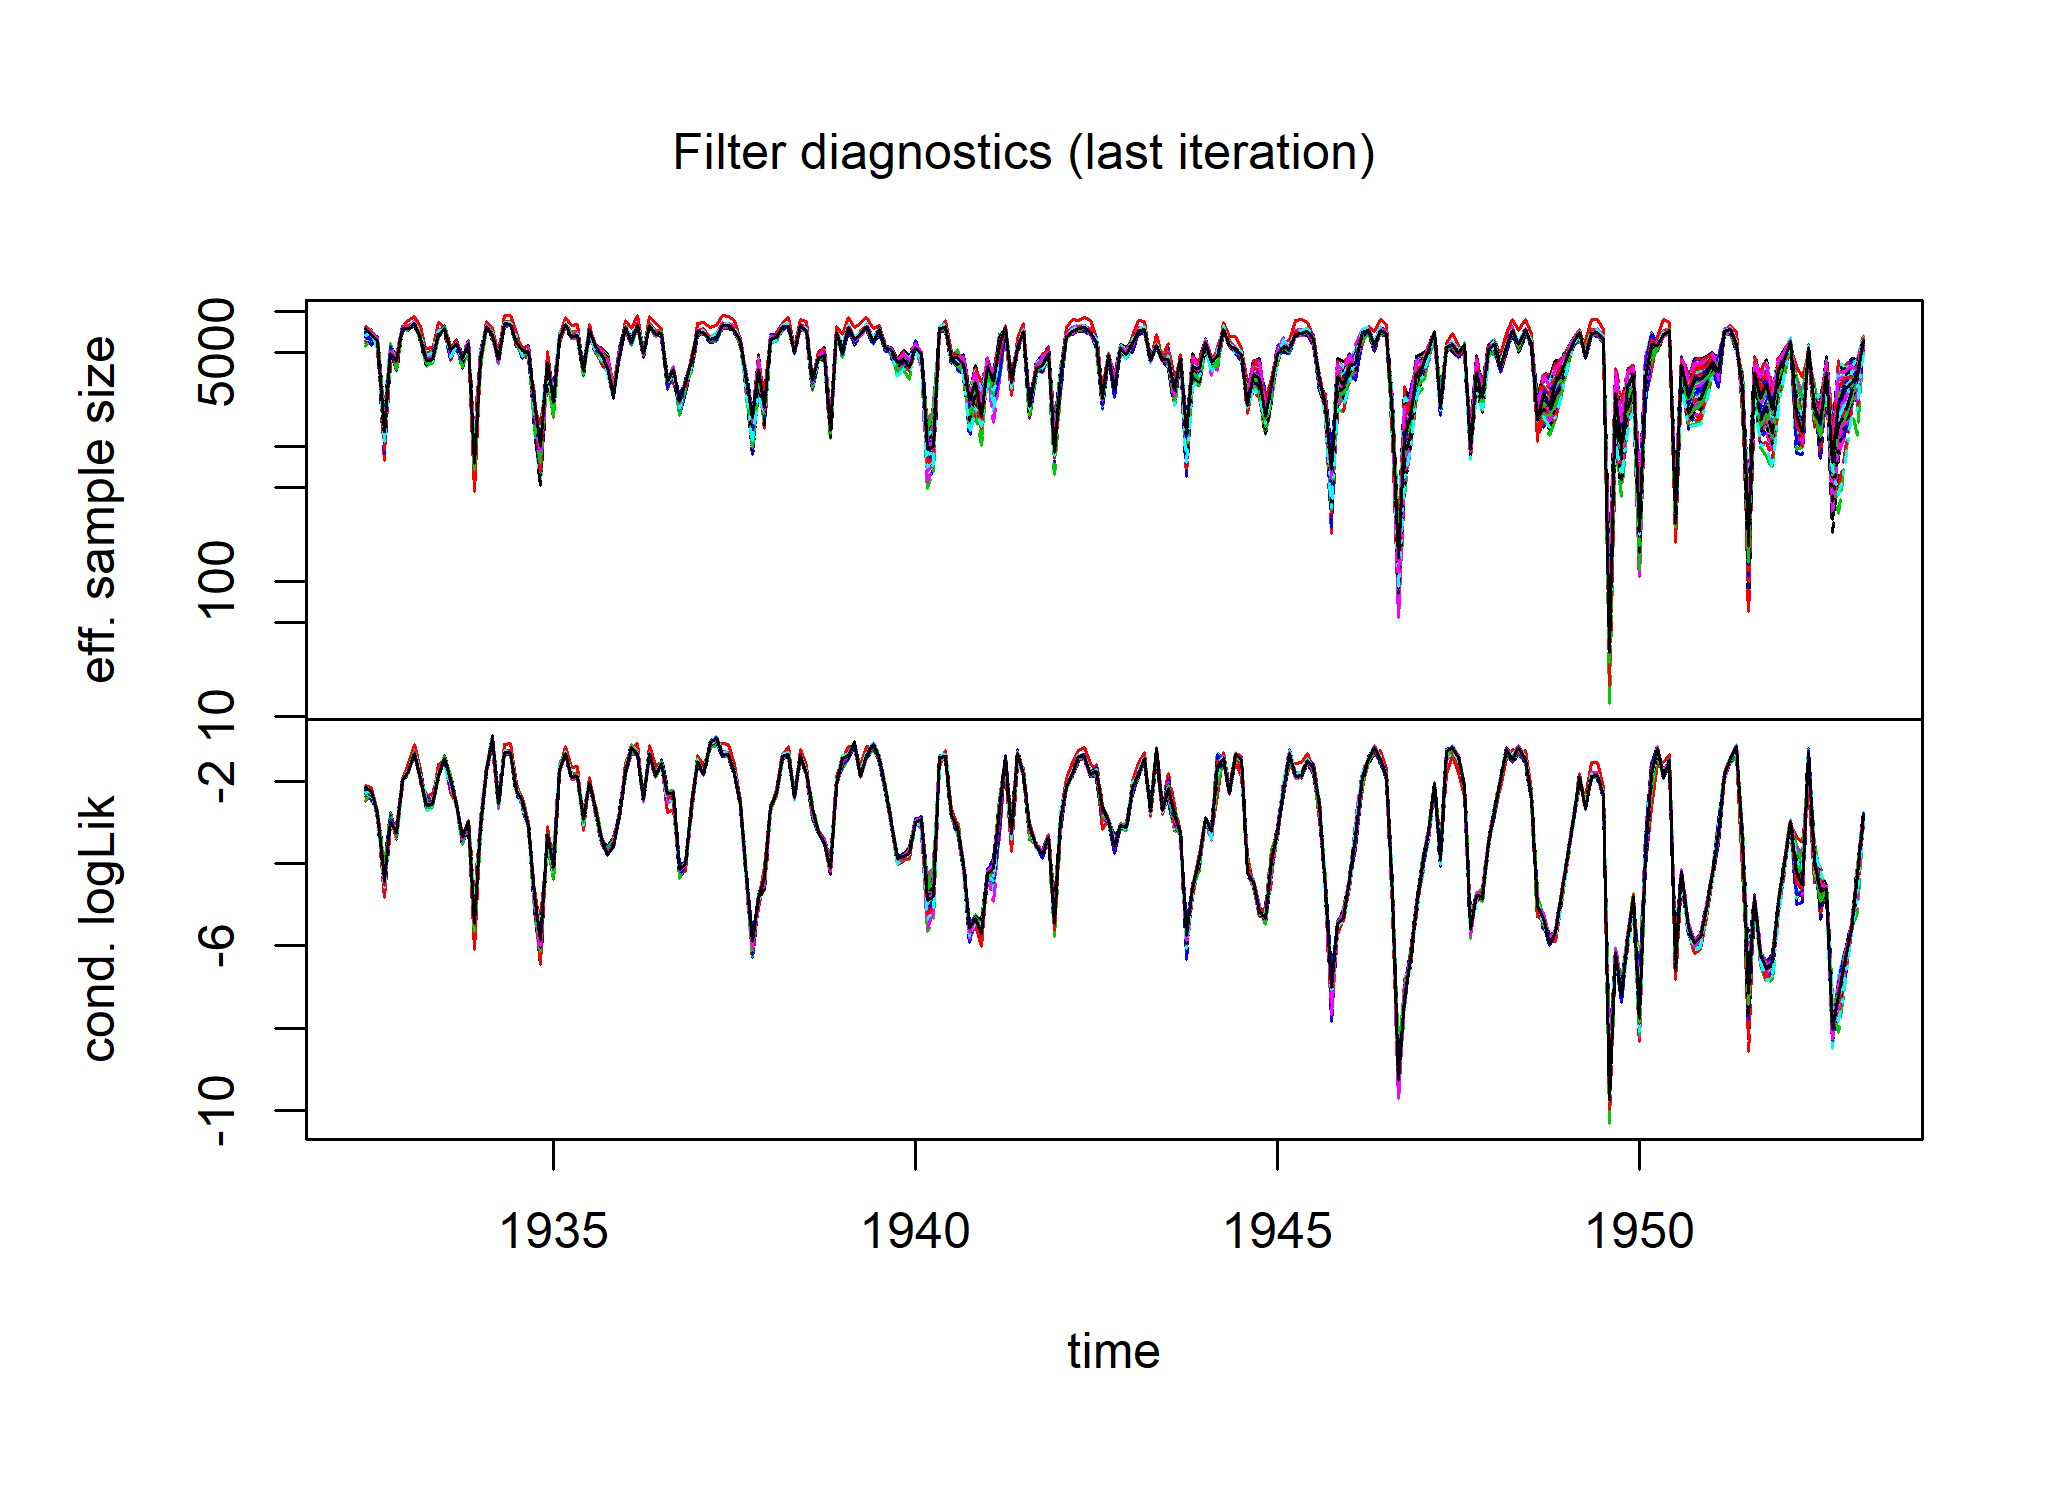
\includegraphics{figure/sp500-mif_diagnostics-1} \end{center}

\begin{center}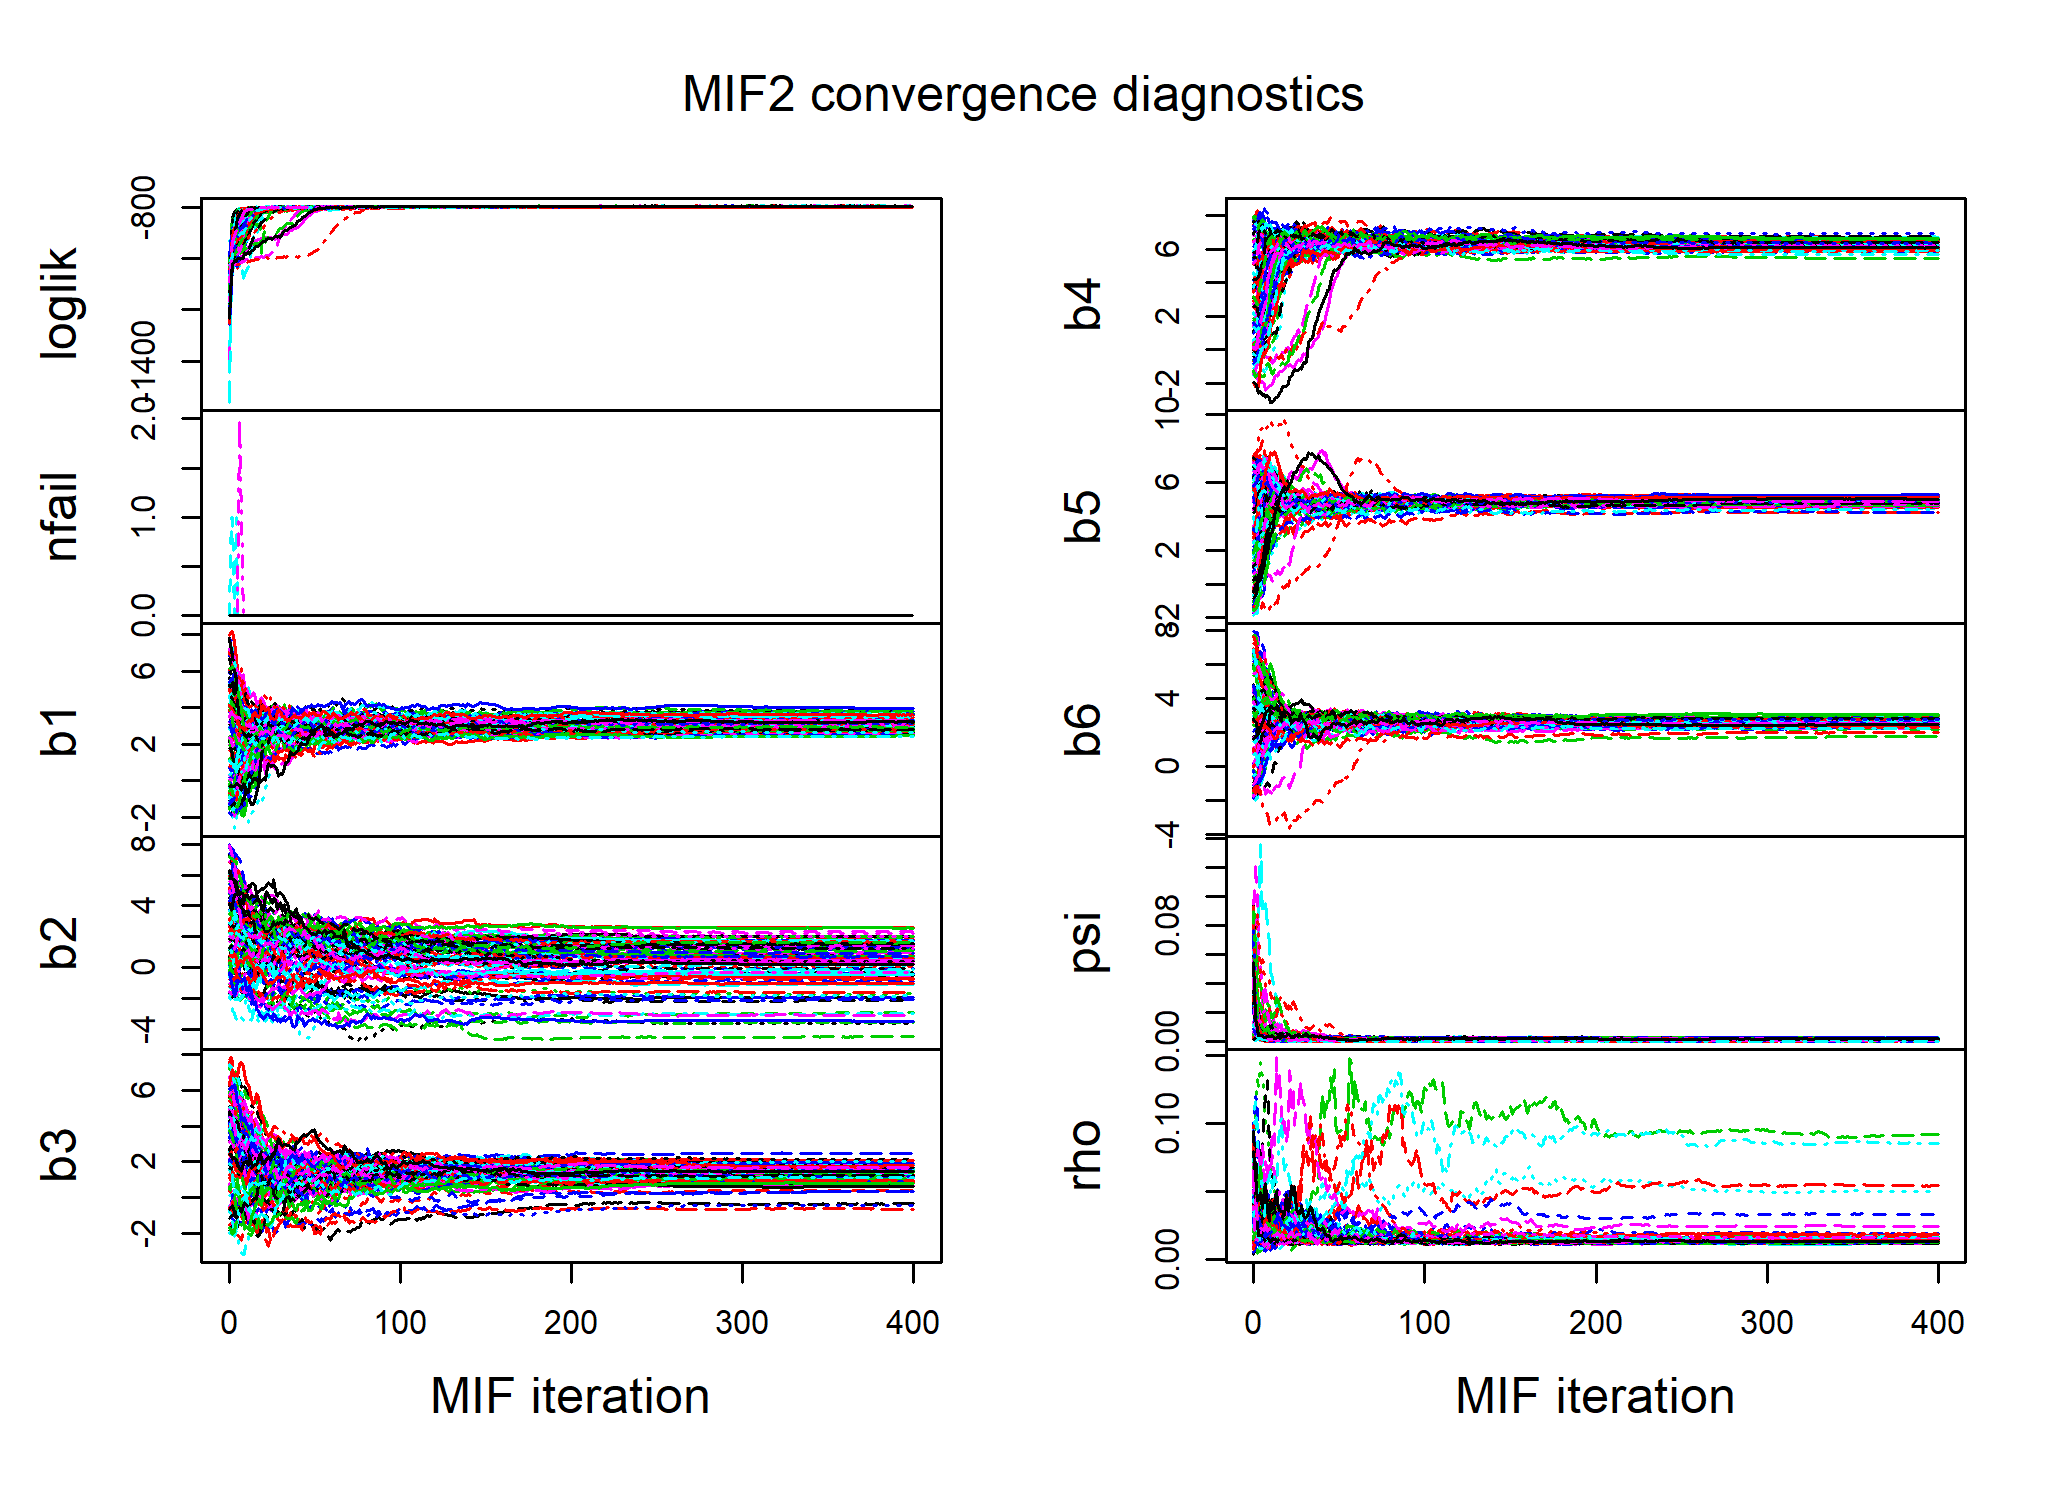
\includegraphics{figure/sp500-mif_diagnostics-2} \end{center}

\begin{center}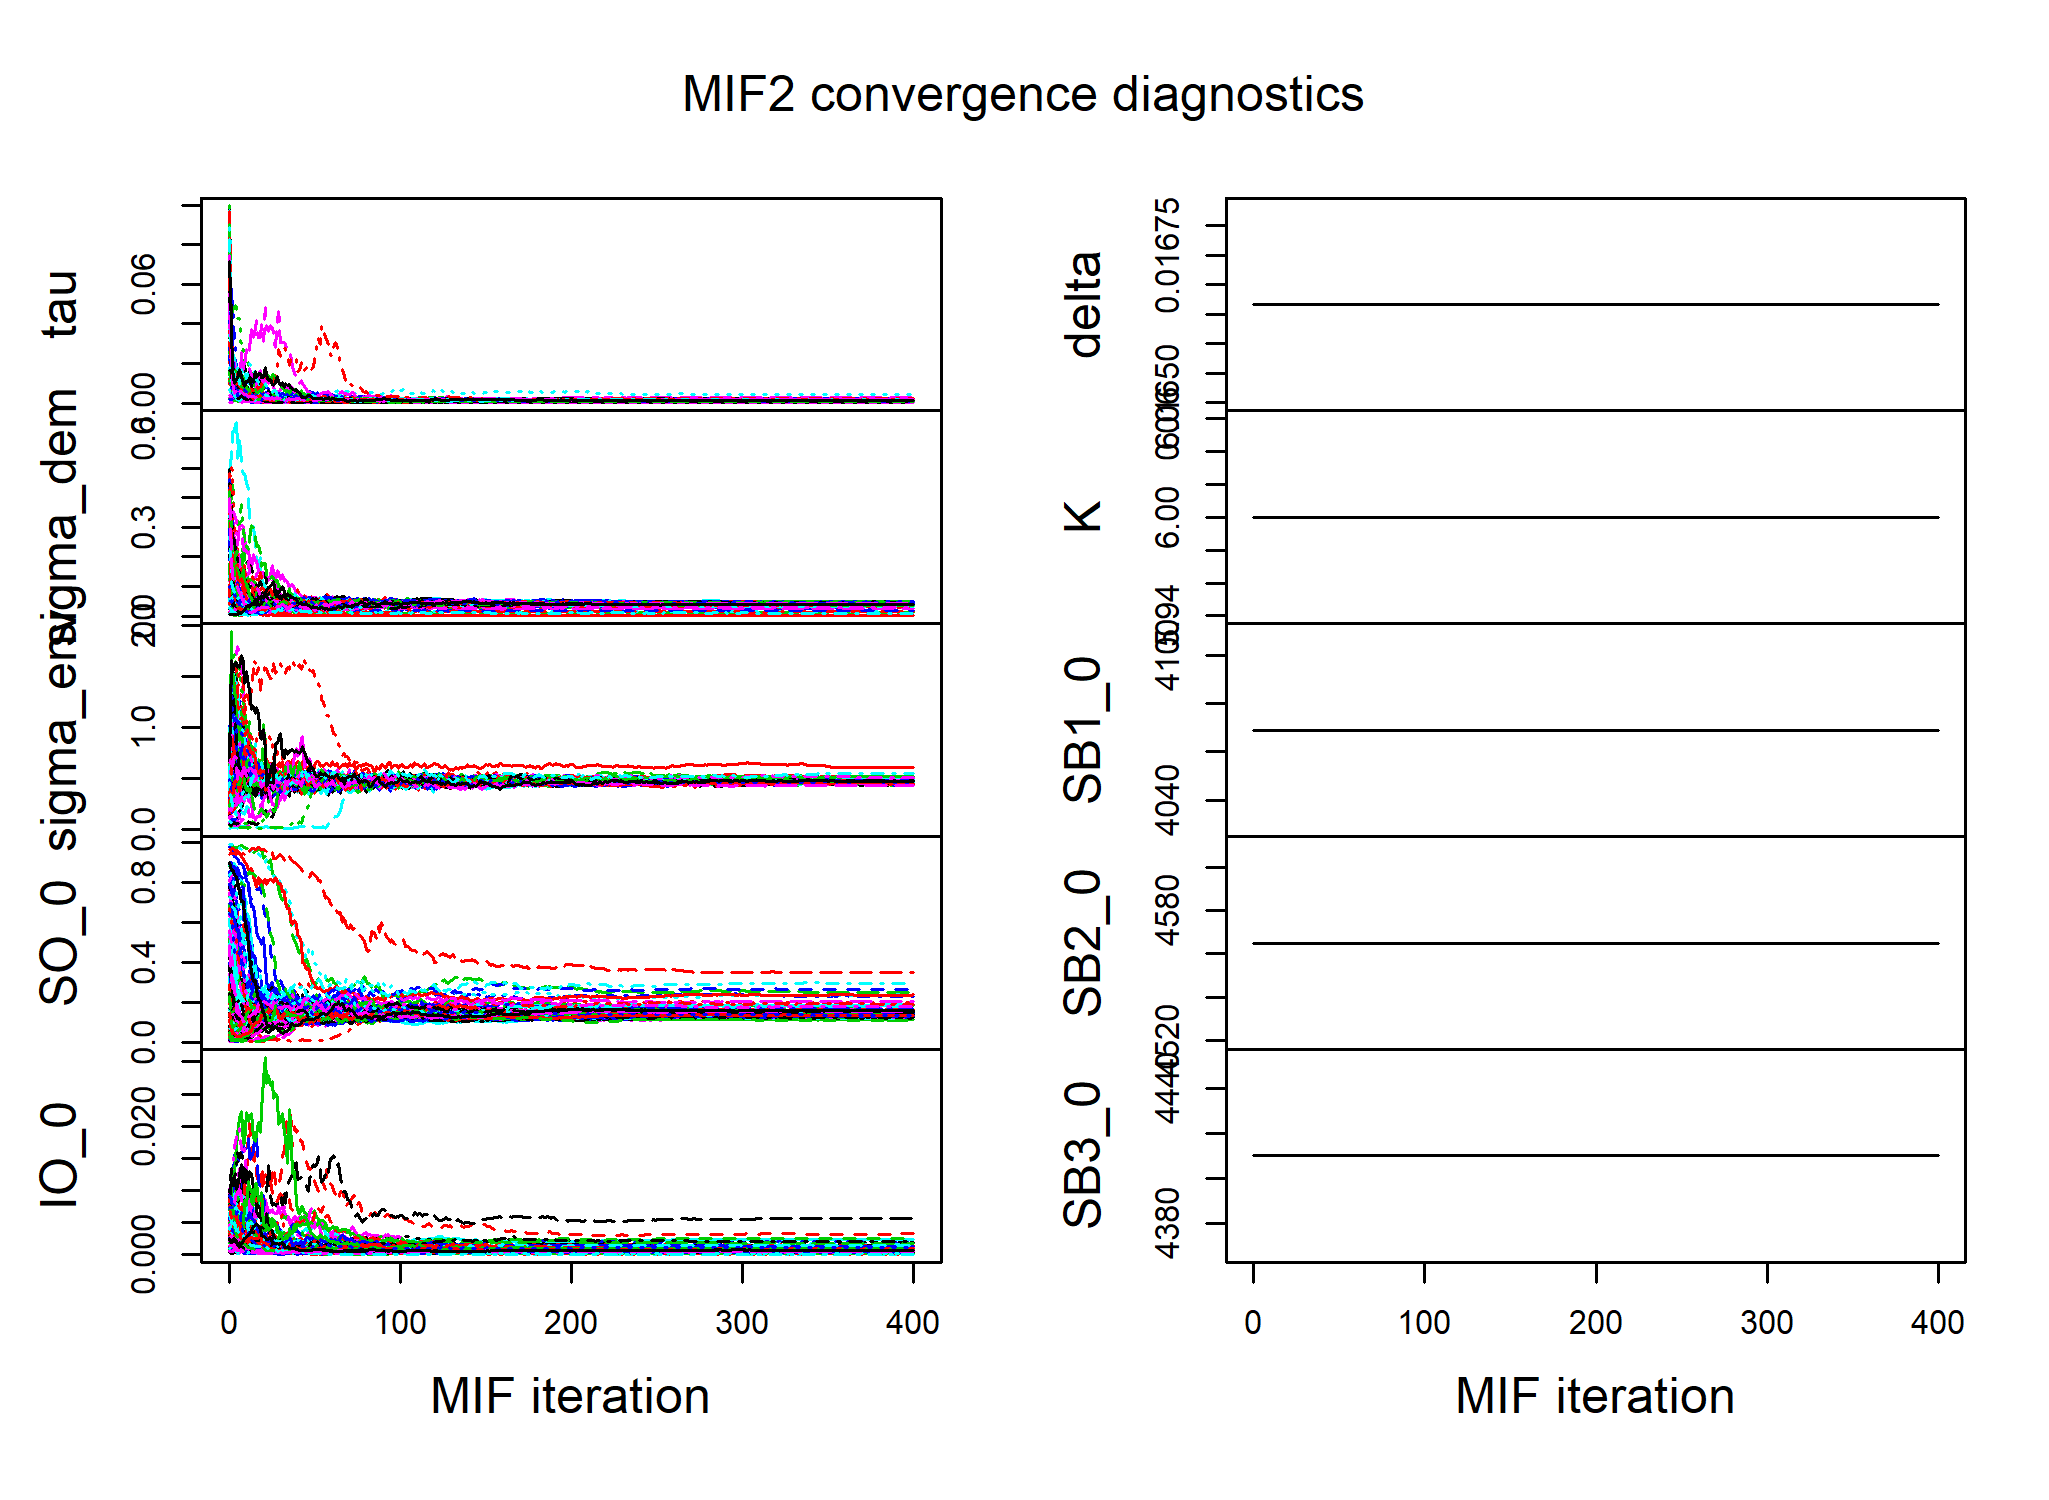
\includegraphics{figure/sp500-mif_diagnostics-3} \end{center}

\begin{center}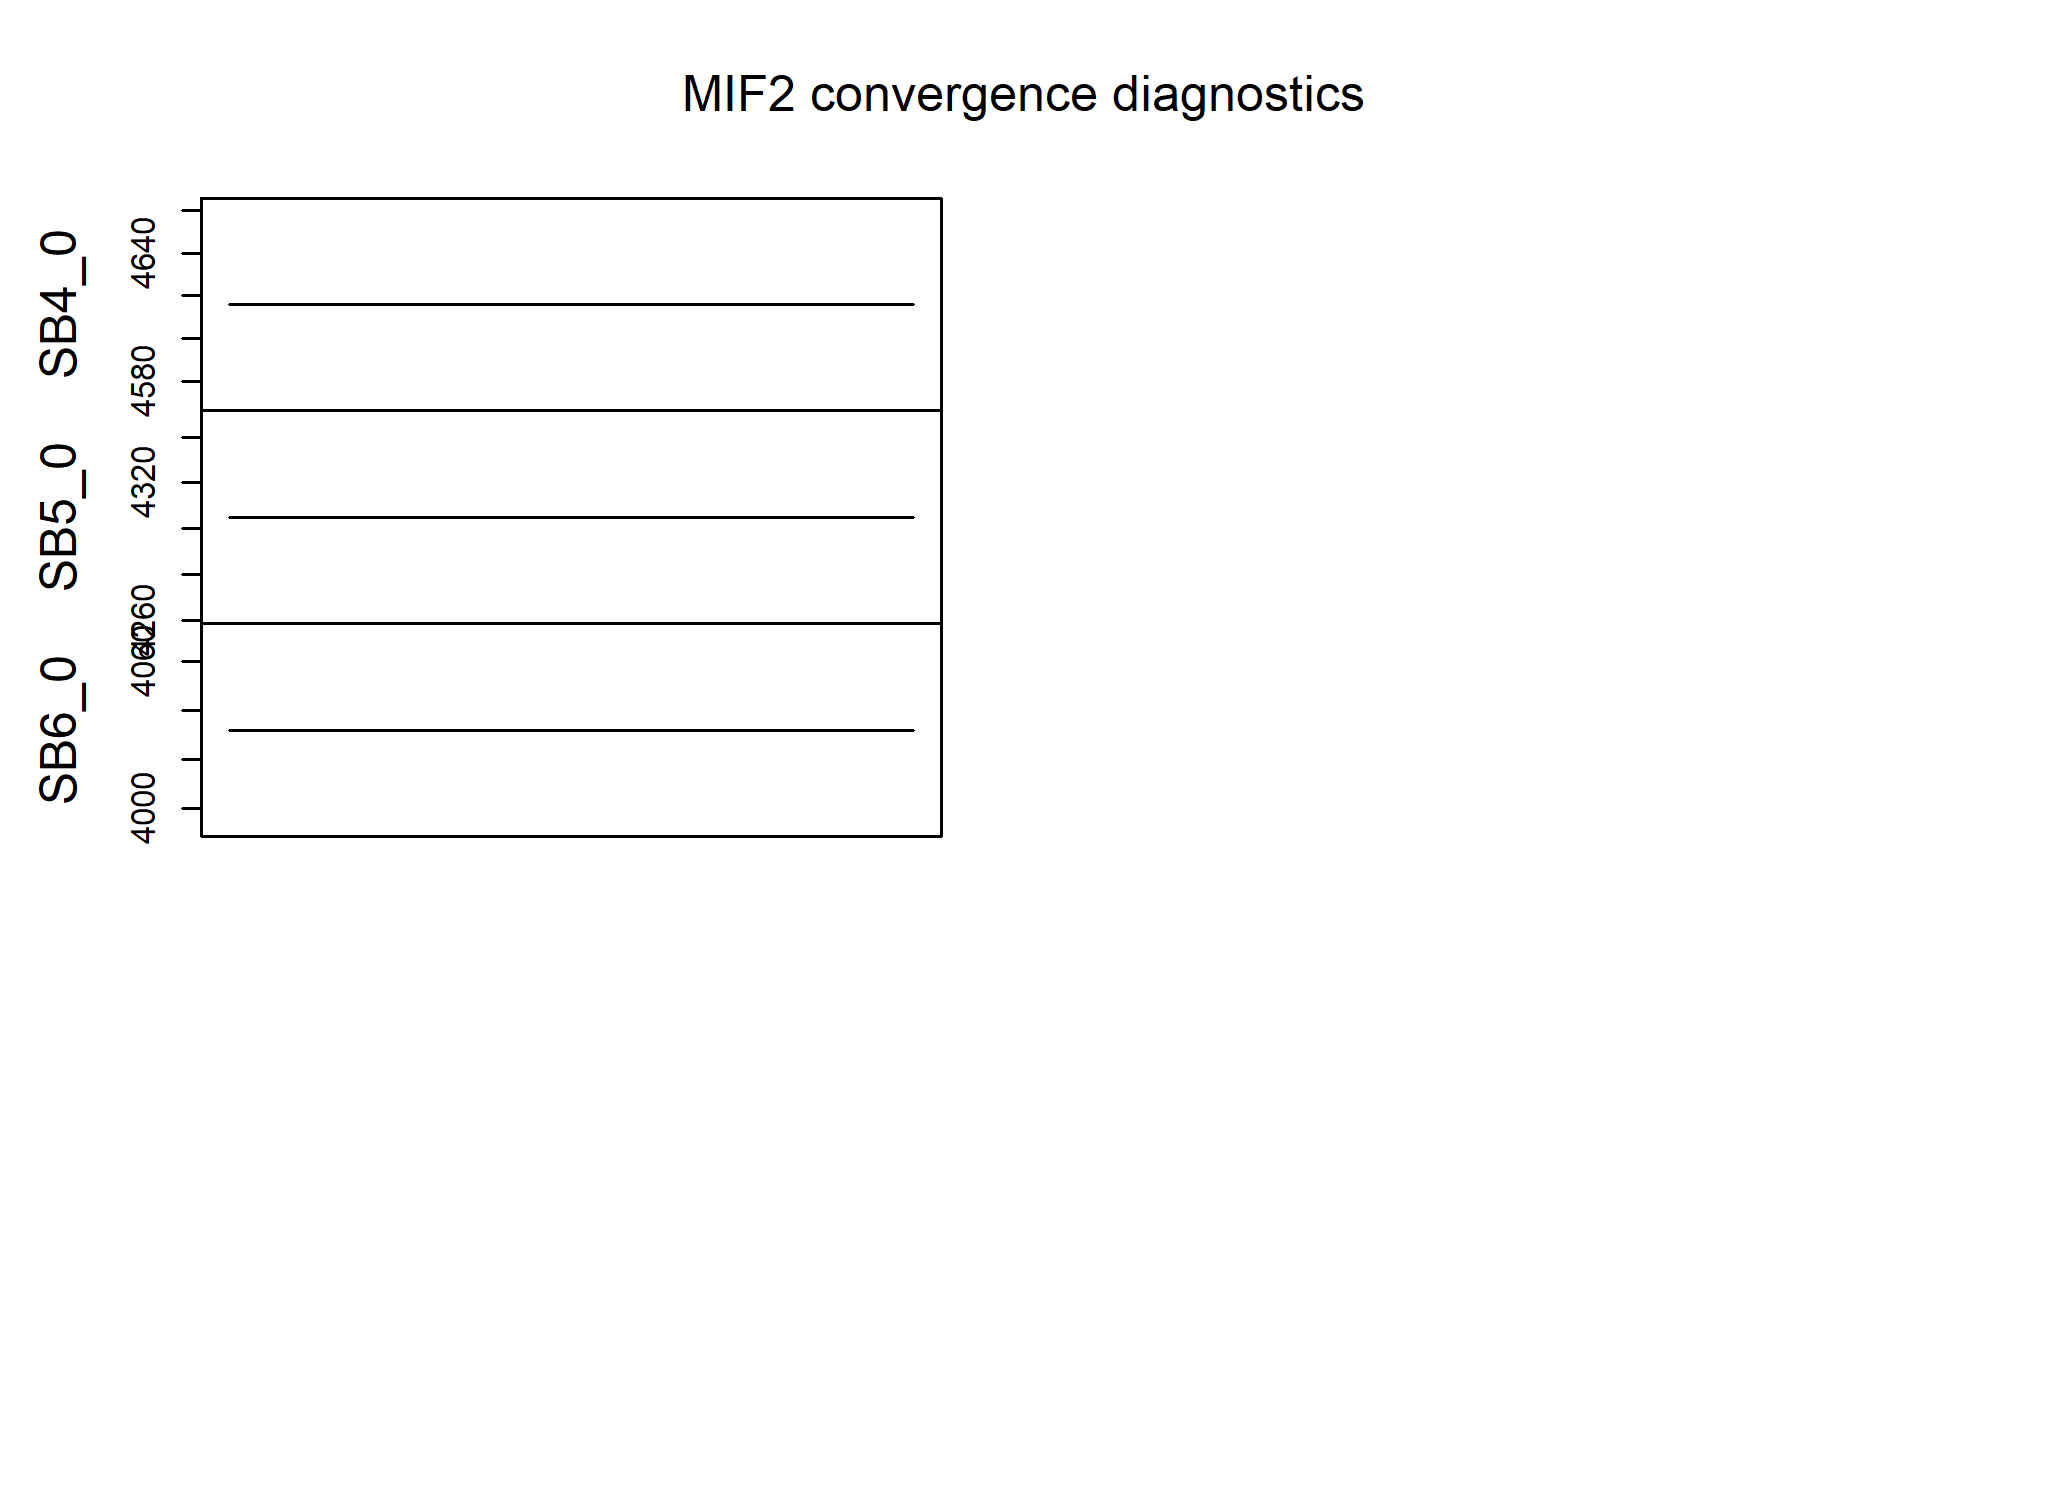
\includegraphics{figure/sp500-mif_diagnostics-4} \end{center}

The likelihood is particularly important to keep in mind. If parameter
estimates are numerically unstable, that could be a consequence of a
weakly identified parameter subspace. The presence of some weakly
identified combinations of parameters is not fundamentally a scientific
flaw; rather, our scientific inquiry looks to investigate which
questions can and cannot be answered in the context of a set of data and
modeling assumptions. Thus, as long as the search is demonstrably
approaching the maximum likelihood region we should not necessarily be
worried about the stability of parameter values (at least, from the
point of diagnosing successful maximization). So, let's zoom in on the
likelihood convergence:

\begin{Shaded}
\begin{Highlighting}[]
\NormalTok{loglik_convergence <-}\StringTok{ }\KeywordTok{do.call}\NormalTok{(cbind,}\KeywordTok{conv.rec}\NormalTok{(m3[r3}\OperatorTok{$}\NormalTok{logLik}\OperatorTok{>}\KeywordTok{max}\NormalTok{(r3}\OperatorTok{$}\NormalTok{logLik)}\OperatorTok{-}\DecValTok{10}\NormalTok{],}\StringTok{"loglik"}\NormalTok{))}
\KeywordTok{matplot}\NormalTok{(loglik_convergence,}\DataTypeTok{type=}\StringTok{"l"}\NormalTok{,}\DataTypeTok{lty=}\DecValTok{1}\NormalTok{,}\DataTypeTok{ylim=}\KeywordTok{max}\NormalTok{(loglik_convergence,}\DataTypeTok{na.rm=}\NormalTok{T)}\OperatorTok{+}\KeywordTok{c}\NormalTok{(}\OperatorTok{-}\DecValTok{10}\NormalTok{,}\DecValTok{0}\NormalTok{))}
\end{Highlighting}
\end{Shaded}

\begin{center}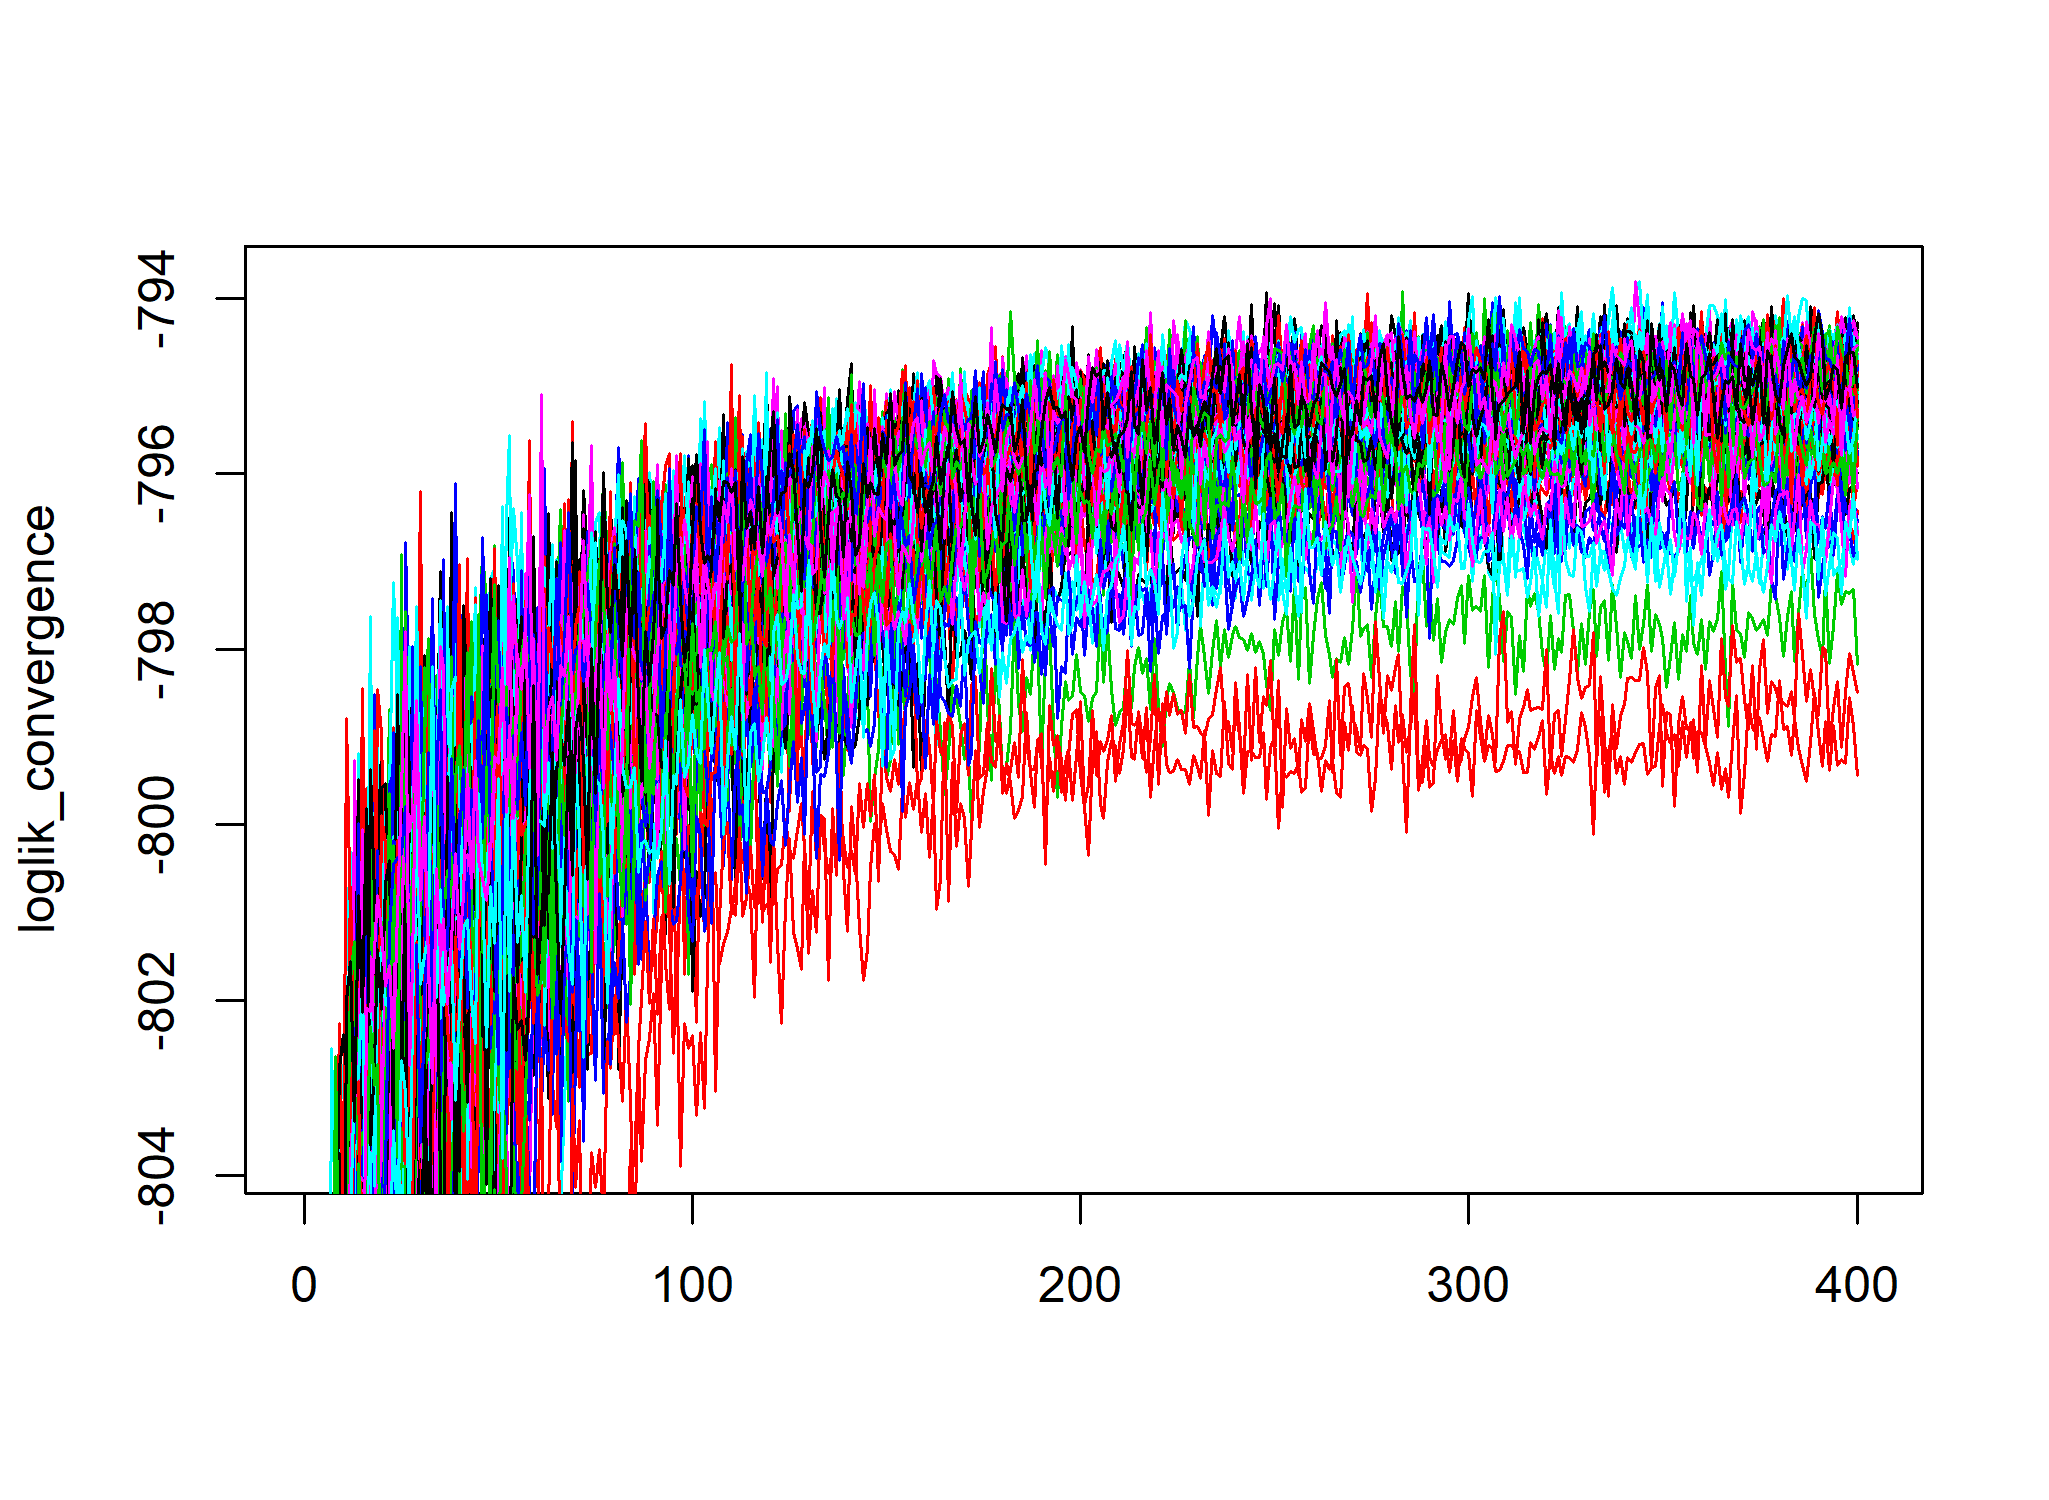
\includegraphics{figure/sp500-likelihood_convergence-1} \end{center}

\begin{center}\rule{0.5\linewidth}{\linethickness}\end{center}

\begin{center}\rule{0.5\linewidth}{\linethickness}\end{center}

Acknowledgment

These notes draw on material developed for a short course on
\href{http://kingaa.github.io/sbied/}{Simulation-based Inference for
Epidemiological Dynamics} by Aaron King and Edward Ionides, taught at
the University of Washington Summer Institute in Statistics and Modeling
in Infectious Diseases, 2015, 2016 and 2017.

\begin{center}\rule{0.5\linewidth}{\linethickness}\end{center}

\subsection*{References}\label{references}
\addcontentsline{toc}{subsection}{References}

\hypertarget{refs}{}
\hypertarget{ref-ionides15}{}
Ionides, E. L., D. Nguyen, Y. Atchadé, S. Stoev, and A. A. King. 2015.
Inference for dynamic and latent variable models via iterated, perturbed
Bayes maps. Proceedings of the National Academy of Sciences of USA
112:719--724.

\hypertarget{ref-martinez-bakker15}{}
Martinez-Bakker, M., A. A. King, and P. Rohani. 2015. Unraveling the
transmission ecology of polio. PLoS Biology 13:e1002172.


\end{document}
